% Document class and styles
\documentclass[10pt,twoside]{classes/csthesis}
\usepackage{style/s5paper}

% Other imported packages
\usepackage{graphicx}
\usepackage[utf8]{inputenc}
\usepackage{lipsum} % For lipsum
\usepackage[final]{pdfpages}
\usepackage{hyperref}
\usepackage{subcaption}
% Packages imported by you
\usepackage{booktabs}
\usepackage{csquotes}
\usepackage{amsmath,amssymb}
\usepackage{xcolor}
\usepackage{textcomp} % To get the copyleft symbol
% Library
\usepackage[backend=biber]{biblatex}
\usepackage{tikz}
\usepackage{amsmath}
\usetikzlibrary{positioning}
\addbibresource{library_sample.bib}

\graphicspath{{images/}}

\DeclareUnicodeCharacter{0301}{\'{e}}

\newcommand{\PaperI}{\Large \textbf{Safety-critical computer vision: an empirical survey of adversarial evasion attacks and defenses on computer vision systems.} \\{}\\ \large Charles Meyers, Tommy L\"{o}fstedt, and Erik Elmroth. \\{}\\ \normalsize Artificial Intelligence Review,  Volume 56, 2023. \\ \\ \emph{To what degree can we trust modern ML models? }}

\newcommand{\paperI}{\textit{Safety-critical computer vision: an empirical survey of adversarial evasion attacks and defenses on computer vision systems.} Charles Meyers, Tommy L\"{o}fstedt, and Erik Elmroth.  Artificial Intelligence Review, Volume 56, 2023. }


\newcommand{\PaperII}{\Large \textbf{Massively parallel evasion attacks and the pitfalls of adversarial retraining. } \\{}\\ \large Charles Meyers, Tommy L\"{o}fstedt, Erik Elmroth  \\{}\\ \normalsize EAI Endorsed Transactions on Internet of Things, Volume 10, 2024 \\ \\\emph{Can we overcome an adversary by generating or using more data?}}

\newcommand{\paperII}{\emph{Massively parallel evasion attacks and the pitfalls of adversarial retraining. } Charles Meyers, Tommy L\"{o}fstedt, and Erik Elmroth. EAI Endorsed Transactions on Internet of Things, Volume 10, 2024. }

\newcommand{\PaperIII}{\Large \textbf{Training Rate and Survival Heuristic for Inference and Robustness Evaluation (Trashfire).} \\{}\\ \large Charles Meyers, Mohammad Reza Saleh Sedghpour, Tommy L\"{o}fstedt, and Erik Elmroth. \\{}\\ \normalsize IEEE International Conference on Machine Learning and Cybernetics (ICMLC): Volume 1, 2024. \\ \\ \emph{How can we formalise the cost benefit relationship between robustness and particular choice of model?}}

\newcommand{\paperIII}{\emph{Training Rate and Survival Heuristic for Inference and Robustness Evaluation (Trashfire).} Charles Meyers, Mohammad Reza Saleh Sedghpour, Tommy L\"{o}fstedt, and Erik Elmroth. IEEE International Conference on Machine Learning and Cybernetics (ICMLC), Volume 1, 2024. }

\newcommand{\PaperIV}{\Large \emph{A Cost-Aware Approach to Adversarial Robustness in Neural Networks.} \\{}\\ \large Charles Meyers, Mohammad Reza Saleh Sedghpour, Tommy L\"{o}fstedt, and Erik Elmroth \\{}\\ \normalsize Submitted for publication September 2024.  \\ \\ \emph{Can we extend the analysis in Paper III to examine the relationship between cost and robustness?}}

\newcommand{\paperIV}{\emph{A Cost-Aware Approach to Adversarial Robustness in Neural Networks.} Charles Meyers, Mohammad Reza Saleh Sedghpour, Erik Elmroth, and Tommy L\"{o}fstedt.  Submitted for publication September 2024. }

\newcommand{\PaperV}{\Large 
\textbf{ A Tiny, Client-Side Classifier.} \\{}\\ \large Charles Meyers, Aaron P. MacSween, Erik Elmroth, and Tommy L\"{o}fstedt. \\{}\\ \normalsize Manuscript, Ume{\aa} University, Sweden, 2024. \\ \\ 
\emph{Is it possible to build a classifier that circumvents the inherent weaknesses of centralised training paradigms?}}

\newcommand{\paperV}{\emph{A Tiny, Client-Side Classifier.} Charles Meyers, Aaron P. MacSween, Erik Elmroth, and Tommy L\"{o}fstedt.   Manuscript, Ume{\aa} University, Sweden, 2024.}

\newcommand{\PaperVI}{\Large 
\textbf{Deckard: A tool for robust, declarative, and reproducible AI.} \\{}\\ \large Charles Meyers. \\{}\\ \normalsize Manuscript, Ume{\aa} University, Sweden, 2025. \\ \\
\emph{How can we build auditable and reproducible tests to meet regulatory standards for safety critical systems?}}

\newcommand{\paperVI}{\emph{Deckard: A tool for robust, declarative, and reproducible AI.} Charles Meyers. Manuscript, Ume{\aa} University, Sweden, 2025. }

% \begin{description}
%     %  Survey Paper
%     \item[R1] To what degree can we trust modern ML models? 
%     %  Massively Parllel
%     \item[R2] Can we overcome an adversary by generating or using more data?
%     %  Trashfire
%     \item[R3] How can we formalise the cost benefit relationship between robustness and particular choice of model?
%     % A Cost-Aware approach (Cloud paper)
%     \item[R4] Can we extend the analysis in R3 to examine the relationship between cost and robustness?
%     %  NCD Paper
%     \item[R5] Is it possible to build a classifier that circumvents the inherent weaknesses of centralised training paradigms?
%     %  Deckard Paper
%     \item[R6] How can we build auditable and reproducible tests to meet regulatory standards for safety critical systems?
    
% \end{description}
% ------------------------------------------------------
% Begin document
% ------------------------------------------------------
\begin{document}

% ------------------------------------------------------
% Front cover
% ------------------------------------------------------
\thispagestyle{empty}
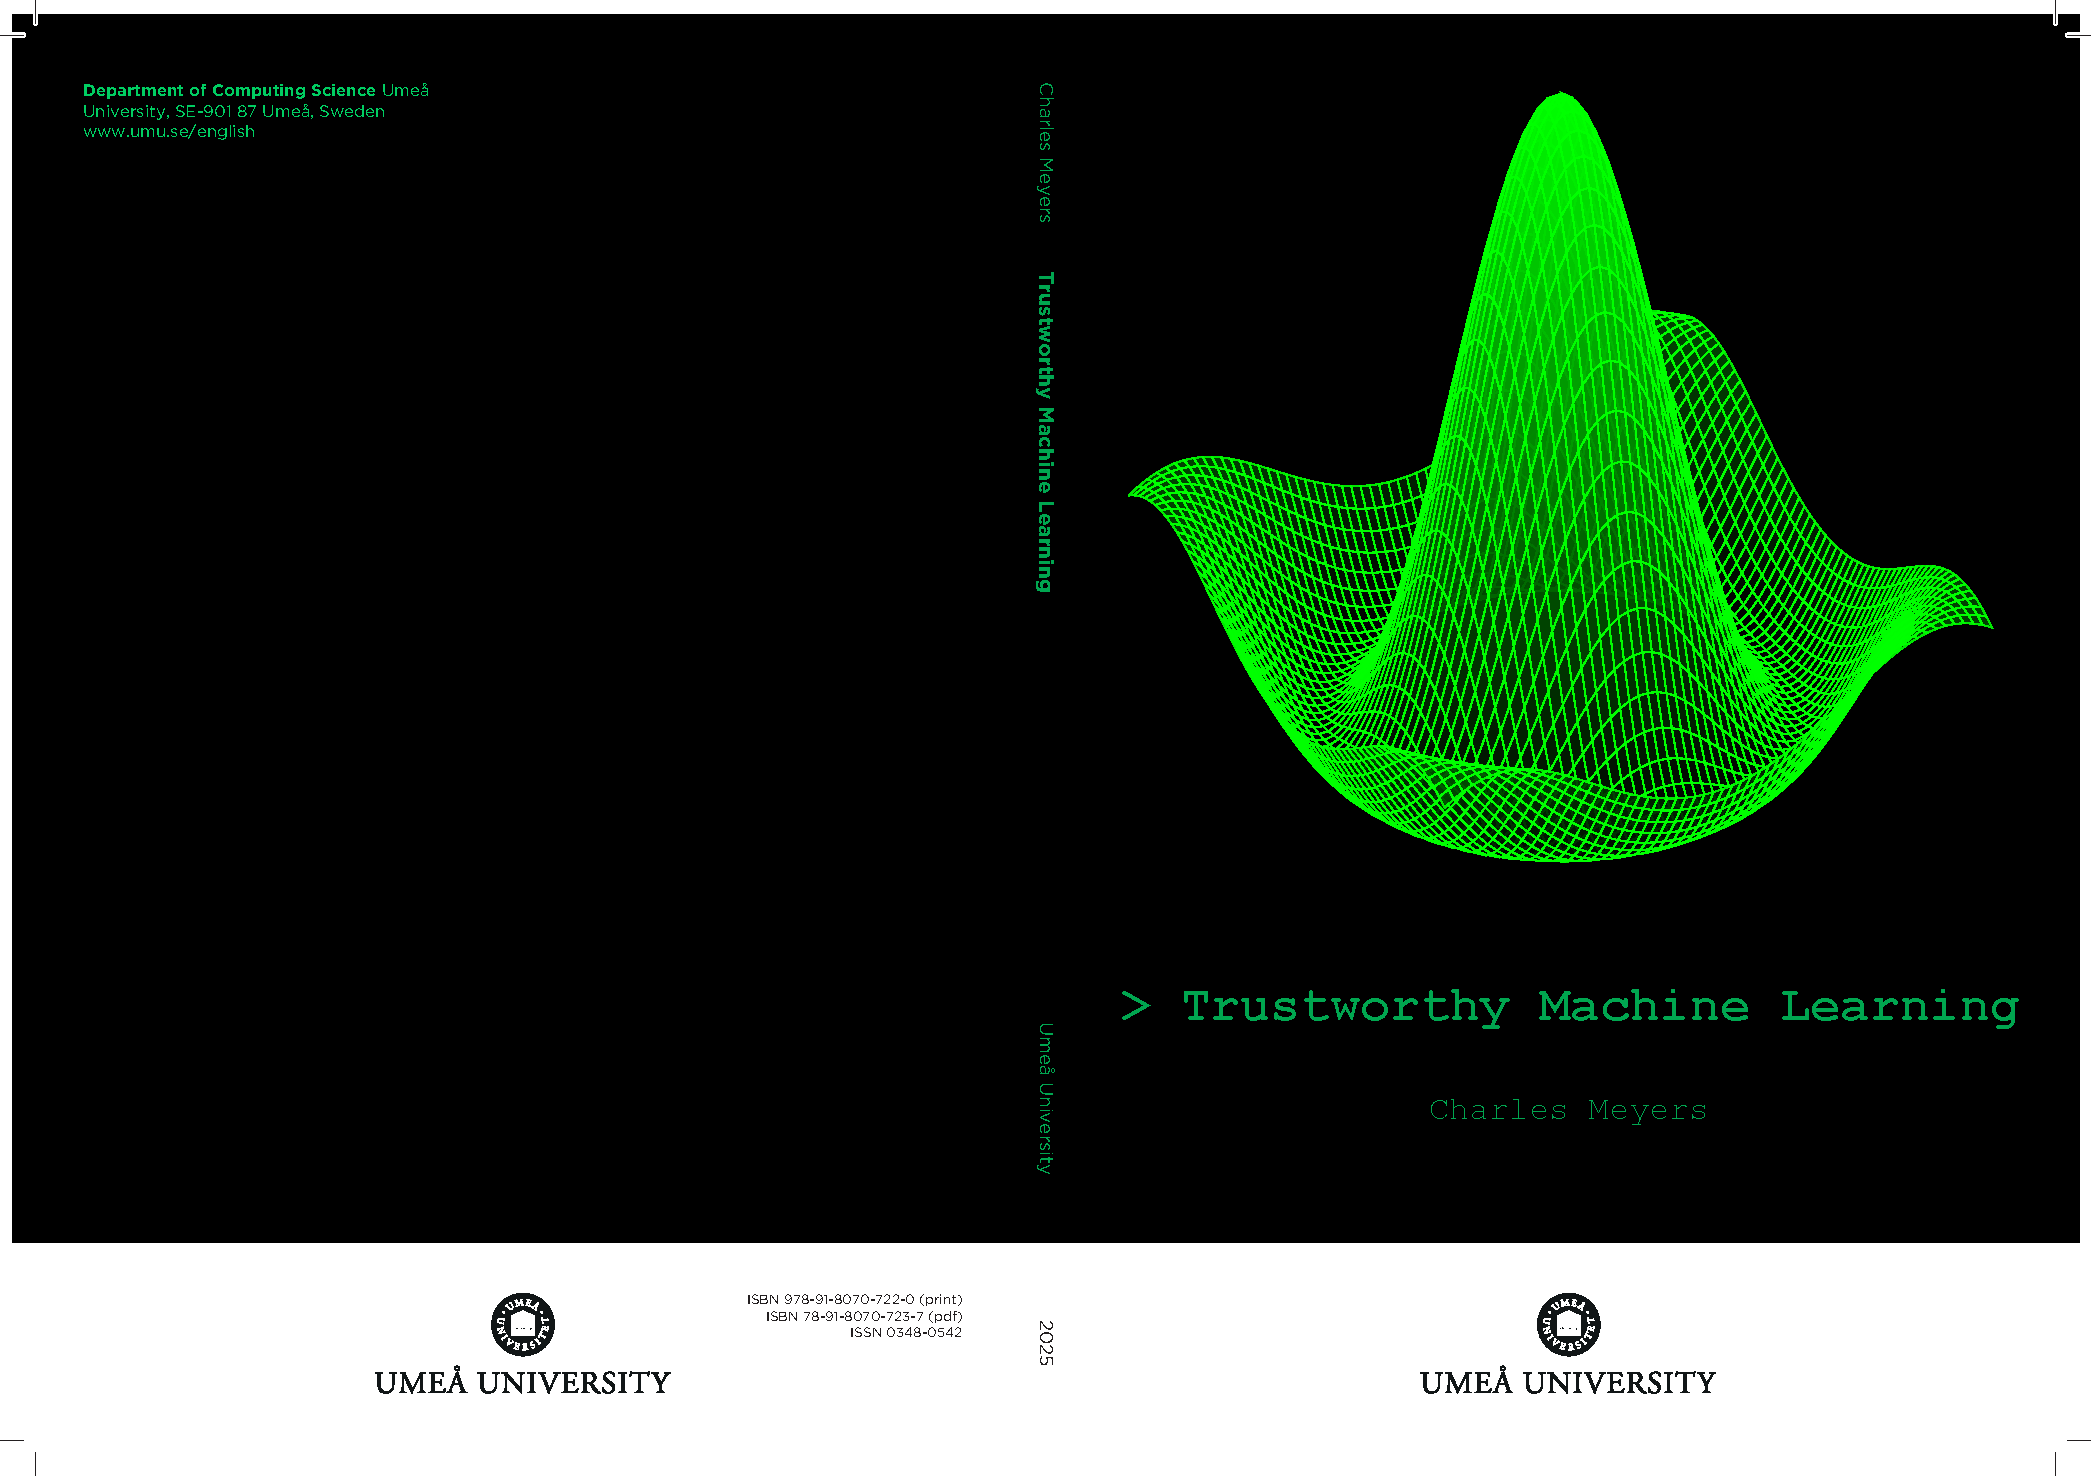
\includepdf[
  trim=180mm 5mm 5mm 5mm,
  clip,
  pagecommand={-},
  width=\paperwidth,
  height=\paperheight,
]{thesis_other_chapters/cover.pdf}



% ------------------------------------------------------
% Pre-pages
% ------------------------------------------------------
\pagenumbering{roman}

\thispagestyle{empty}

\mbox{}

\vskip 40pt
\begin{center}
  {\huge \bfseries Trustworthy Machine Learning \par}
  \vskip 3em
  {\Large
    \lineskip .75em
    \begin{tabular}[t]{c}
      {\it Charles Meyers}
    \end{tabular}\par}
  \vskip 3em
  \noindent% \parbox[b][17mm][c]{.5\linewidth}
  \vskip 15em
  
\includegraphics[height=25mm]{images/umu-logo-SE.png}
  \vskip 3em

\noindent% \parbox[b][17mm][c]{.5\linewidth}
{
%\begin{large}
\scshape
Doctoral Thesis, May 2025\\
Department of Computing~Science\\
Ume{\aa} University\\
Sweden
%\end{large}
}
\hfill
\end{center}


\newpage

\thispagestyle{empty}
$ $

\vfill

\noindent\begin{minipage}{\textwidth}
Department of Computing Science\\
Ume{\aa} University\\
SE-901 87  Ume{\aa}, Sweden

\vspace{10pt}

\emph{cmeyers@cs.umu.se}

\vspace{1pt}

This work is protected by the Swedish Copyright Act (1960:729) \\
\copyright~Copyright reserved by Charles Meyers, 2025\\
\begin{tabbing}

\footnotesize
Except \=\footnotesize Paper I \copyright~Springer, 2023 \\
   \>\footnotesize Paper II, \copyright~EAI, 2024  \\
   \>\footnotesize Paper III, \copyright~IEEE, 2024  \\



\end{tabbing}


\footnotesize All text, images, data, and linked source code are distributed under CC-BY-NC-SA~\textcopyleft .

\vspace{5pt}

{\bfseries
ISBN (print) 978-91-8070-722-0\\
ISBN (digital) 978-91-8070-723-7\\
ISSN 0348-0542\\
UMINF 25.10}

\vspace{10pt}

Printed by Scandinavian Print Group, 2025
\end{minipage}

\cleardoublepage

\chapter*{Abstract}

This thesis studies adversarial robustness, privacy, and reproducibility in safety-critical machine learning systems, with particular emphasis on computer vision, anomaly detection, and evasion attacks through a series of papers.
The work begins by analysing the practical costs and benefits of defence strategies against adversarial attacks, revealing that common robustness metrics are poor indicators of real-world adversarial performance (Paper I). 
Through large-scale experiments, it further demonstrates that adversarial examples can often be generated in linear time, granting attackers a computational advantage over defenders (Paper II).
To address this, a novel metric—the Training Rate and Survival Heuristic (TRASH)—was developed to predict model failure under attack and facilitate early rejection of vulnerable architectures (Paper III).
This metric was then extended to real-world cost, showing that adversarial robustness can be improved using low-cost, low-precision hardware without sacrificing accuracy (Paper IV).

Beyond robustness, the thesis tackles privacy by designing a lightweight, client-side spam detection model that preserves user data and resists several classes of attacks without requiring server-side computation (Paper V).
Recognizing the need for reproducible and auditable experiments in safety-critical contexts, the thesis also presents \texttt{deckard}, a declarative software framework for distributed and robust machine learning experimentation (Paper VI).

Together, these contributions offer empirical techniques for evaluating and improving model robustness, propose a privacy-preserving classification strategy, and deliver practical tooling for reproducible experimentation. 
Ultimately, this thesis advances the goal of building machine learning systems that are not only accurate, but also robust, reproducible, and trustworthy.

\chapter*{Sammanfattning}

Denna avhandling studerar robusthet, integritet och reproducerbarhet i säker\-hetskritisk maskininlärning, med särskild tonvikt på datorseende, avvikelse\-detektering och undvikande attacker.

Arbetet inleds med att analysera de praktiska kostnaderna och fördelarna med försvarsstrategier mot attacker, vilket visar att vanliga mått på robusthet är dåliga indikatorer på verklig prestanda i attacker (Artikel~I).
Genom storskaliga experiment visar arbetet vidare att exempel på attacker ofta kan genereras i linjär tid, vilket ger angripare en beräkningsfördel gentemot försvar\-are (Artikel~II).
För att hantera detta presenterar avhandlingen ett nytt mått – Training Rate and Survival Heuristic (TRASH) – för att förutsäga modellfel under attack och underlätta tidigt avvisande av sårbara arkitekturer (Artikel~III).
Detta mått utvidgades sedan till verkliga kostnader, vilket visar att robusthet i attacker kan förbättras med hjälp av billig hårdvara med låg precision utan att offra noggrannheten (Artikel~IV).

Utöver robusthet behandlar avhandlingen integritet genom att utforma en lättviktig klientbaserad modell för spamdetektering som bevarar användardata och står emot flera klasser av attacker utan att kräva att beräkningar görs på serversidan (Artikel~V).
Som svar på behovet av reproducerbara och gransk\-ningsbara experiment i säkerhetskritiska sammanhang presenterar avhandlingen även \texttt{deckard}, ett deklarativt programvaruramverk för distribuerade och robusta maskininlärningsexperiment (Artikel~VI).

Tillsammans erbjuder dessa bidrag empiriska tekniker för att utvärdera och förbättra modellers robusthet, föreslår en integritetsbevarande klassificeringsstrategi och levererar praktiska verktyg för reproducerbara experiment.
Sammantaget främjar avhandlingen målet att bygga maskininlärningssystem som inte bara är korrekta, utan också robusta, reproducerbara och pålitliga.
\cleardoublepage

\chapter*{Preface}
This thesis is based on the following papers:

\begin{paperlist}
    \item Meyers, Charles, Tommy L\"{o}fstedt, and Erik Elmroth.``Safety-critical computer vision: an empirical survey of adversarial evasion attacks and defenses on computer vision systems.''
    \em{Artificial Intelligence Review (2023): Volume 56. Pages 217-251.} 
    \\
    Available online: 
    \\\href{https://link.springer.com/content/pdf/10.1007/s10462-023-10521-4.pdf}{
    https://link.springer.com/content/pdf/10.1007/s10462-023-10521-4.pdf}
    
    \item Meyers, C., L\"{o}fstedt, T., and Elmroth, E. (2024)
    Massively parallel evasion attacks and the pitfalls of adversarial retraining. 
    \em{EAI Endorsed Transactions on Internet of Things, Volume 10. Published by EAI.} 
    \\
    Available online:
    \\
    \href{https://publications.eai.eu/index.php/IoT/article/view/6652}{https://publications.eai.eu/index.php/IoT/article/view/6652}

    \item C. Meyers, M. R. S. Sedghpour, T. L\"{o}fstedt, and E. Elmroth,``A Training Rate and Survival Heuristic for Inference and Robustness Evaluation (Trashfire), 
    \em{2024 International Conference on Machine Learning and Cybernetics (ICMLC).}
    \\
    Available online:
    \\
    \href{https://ieeexplore.ieee.org/document/10935101}{https://ieeexplore.ieee.org/document/10935101}
    \\
    Open access preprint:
    \href{https://arxiv.org/abs/2401.13751}{https://arxiv.org/abs/2401.13751}
    


    \item Charles Meyers, Mohammad Reza, Tommy L\"{o}fstedt, and \\ Erik Elmroth.``A Cost-Aware Approach to Adversarial Robustness in Neural Networks. Under Review since September 2024''
    \\
    Open-access preprint: 
    \href{https://arxiv.org/abs/2409.07609}{https://arxiv.org/abs/2409.07609}
    

    \item Charles Meyers, Aaron MacSween, Tommy L\"{o}fstedt, and \\ Erik Elmroth.``A Tiny, Client-Side Classifier.''
    \newblock {\em {Journal, year. page numbers.}}

    \item Charles Meyers.``Deckard: A tool for robust, declarative, and reproducible AI.''
    \newblock {\em{Journal, year. page numbers.}}
    
\end{paperlist}



\section*{Funding Statement}

Financial support has been provided in part by the Knut and Alice Wallenberg Foundation grant number 2019.0352 and by the eSSENCE Programme under the Swedish Government's Strategic Research Initiative.
\cleardoublepage

\chapter*{Acknowledgements}

The first thanks go to Tommy and Erik, my PhD advisors, for guiding me through this whole process and offering feedback that was occasionally encouraging, frequently humbling, and always technically correct. 
Endless thanks also to my colleagues in the Autonomous Distributed Systems Laboratory for the thoughts they inspired, the questions they raised, and the stubborn determination they provoked.

By no means did I get here alone, and I’d like to thank some educators who spent countless hours dragging me this far: Christie Calloway, who somehow managed to inject her awe of mathematics into middle school students; Jonathan Williams, who looked the other way while I spent Algebra class programming on a TI-83 instead of solving for $x$; Lenora Murray, who ran our high school math club, taught me statistics, and repeatedly entrusted a teenage me with vaguely-supervised travel; Dr. Samar ElHitti, who taught me linear algebra and convinced the university to give me unrestricted use of their super-computer; Dr. Johann Thiel, who taught me optimisation and modelling and kept the college math club alive with free pizza; and  
Dr. Viviana Acquavia, for insisting that I finish what I started.

To some colleagues who deserve equal parts praise and apology:
Dr. Abel Souza, for insisting I use a modern development environment and gifting me his lease; Dr. Mohammad Reza, for contributions regarding the mystical realm of ``the cloud''; Dr. Aryaman Jal (and, let’s be honest, Tommy too), for tolerating my mathematical notation long enough to figure out what I was trying to say; and Aaron MacSween, who kept me grounded by asking the important questions---usually variations of ``why are you doing this again?''

A very special thanks goes to Samantha Wolff, Forrest Crellin, Félix Barbut, Domenique André, and Suga the Cat for their years of dedicated service in enabling my relaxation, socialisation, and, most importantly, procrastination. 

Finally, I must thank my family – for the genetic material, for access to early childhood reading material, and for motivating questions like, ``When are you going to find a `real' job?'' and `Can you help me fix my internet?'''

Y'all made this possible. Well, at least, you made it bearable. 

Thanks.

\section*{Funding Statement}

Financial support has been provided in part by the Knut and Alice Wallenberg Foundation grant number 2019.0352 and by the eSSENCE Programme under the Swedish Government's Strategic Research Initiative.

% \section*{Licenses and Copyright}
% TODO: Not sure where to put the Creative Commons notifications. I think I should have it on the relevant title page as well as a summary somewhere. thoughts?
\cleardoublepage

\chapter*{Glossary}

\begin{description}
    % --- Data Concepts ---
    \item[Sample] A single data point or observation, typically consisting of one or more features and, in supervised learning, a label (think: rows in a spreadsheet).
    \item[Feature] An individual measurable property or characteristic of the data used by a model to make predictions (think: columns in a spreadsheet).
    \item[Training set] A collection of data used to teach a machine learning model how to make predictions.
    \item[Validation set] A subset of the data used to tune hyper-parameters and monitor the model's performance during training without affecting the final evaluation.
    \item[Testing set] A separate set of data used to evaluate how well the model performs on new, unseen inputs.
    \item[Label] Either the predicted or ground truth for a given sample. 
    For classification problems, this is a category like ``cat'' or ``dog'', often represented as a binary list with each class having one entry in said list. 
    For regression problems, this is one or more numerical values.
    % --- Models and Model Types ---
    \item[Model] Model: A machine learning model consists of two main parts: a function that maps inputs to outputs (called a hypothesis function), and a way to measure how well it performs (called a loss function). Together, these components allow the model to learn patterns from data and make predictions or decisions on new inputs.
    \item[Classifier] A type of model that assigns input data to one of several predefined categories or classes.
    \item[Regressor] A type of model that assigns one or more numeric output values to a set of input data.
    % --- Parameters and Training Process ---
    \item[Model Parameter] An internal value adjusted during training that helps the model improve its predictions.
    \item[Hyper-parameter] A predefined setting that controls how the model behaves during training or evaluations, such as the learning rate or the number of layers.
    \item[Optimisation] The process of adjusting the model’s internal parameters in order to minimize error and improve performance based on a chosen loss function.
    \item[Training] The process of teaching a machine learning model by providing it with data (a training set) and adjusting its parameters through optimization to minimize errors in predictions.
    % --- Evaluation and Validation ---
    \item[Accuracy] The fraction of correct predictions made by the model out of all predictions.
    \item[Failure Rate] The number of expected number of failures over time.
    \item[Time to Failure] The duration a system operates before a critical error occurs.
    \item[Survival time] The length of time a system continues to function correctly before experiencing a failure.
    \item[Cross-Validation] A method for evaluating model performance by repeatedly dividing the dataset into parts, training the model on some parts and testing it on the remaining parts to ensure generalisation.
    % --- Mathematical Foundations ---
    \item[Distance] A numerical measure of how different or similar two pieces of data are from each other, interpreted geometrically as the space between points.
    \item[Metric Space] A set in which distances between any two points can be consistently measured.
    \item[Linear] A relationship between variables that can be described using a straight line.
    \item[Linearly Separable] A condition where a straight line (or hyperplane in higher dimensions) lie on different sides of this plane.
    \item[Kernel] A mathematical function that allows computing the inner products in a higher-dimensional space without explicitly determining the coordinates in that space, often used in kernel  machines.
    \item[Gradient] A vector that points in the direction of the steepest increase of a function and is used to guide model parameter updates during training.
    % --- Reliability and Risk ---
    \item[Robustness] The ability of a model to maintain performance when facing unusual, noisy, or slightly changed inputs.
    \item[Reliability] The consistency with which a model or system performs its intended function correctly.
    \item[Safety-Critical] Refers to applications where incorrect model behaviour could lead to harm or serious consequences.
    \item[Security] The protection of a model or system from unauthorized access, manipulation, or attacks.
    \item[Privacy] The principle that individuals’ personal information—-such as their identity, behaviour, or sensitive attributes—-should be protected and not revealed by the model, either directly or indirectly, through its predictions or outputs.
    \item[Generalisation Gap] The difference in performance between the training data and real-world data, which indicates how well the model can generalise.
    \item[Fairness] The degree to which a model’s decisions are free of unjust discrimination across different groups or individuals.
    % --- Adversarial Context ---
    \item[Attack] A deliberate strategy used to induce undesired behaviour in a piece of software (\textit{e.g.}, a machine learning model).
    \item[Defence] A method or mechanism designed to protect a model from attacks or to reduce the harm caused by attacks.
    \item[Adversarial Input] Describes inputs specifically designed to deceive or confuse a machine learning model.
    \item[Benign Input] Describes inputs that are natural, expected, and not intended to deceive the model.
\end{description}


\cleardoublepage

\tableofcontents
\cleardoublepage

% ------------------------------------------------------
% Begin actual content
% ------------------------------------------------------
\pagenumbering{arabic}

\include{ch_1_introduction}

\include{ch_2_safety}

\chapter{Machine Learning}
\label{ch:ml}
Machine learning is a branch of mathematics and computer science that attempts to build models that can learn from data and/or generalise to unseen data to perform a task without explicit instructions, and the specific term dates back to 1959~\cite{samuel1959some}. 

While many other models have been proposed, it's not necessary to exhaustively enumerate them here. 
For a comprehensive study of the matter, see ``Understanding Machine Learning''~\cite{shalev2014understanding}. 
However, a subset of models is outlined below to now only introduce the models used throughout the text, but to develop an intuition about the various considerations of an ML model and the resultant limitations. 
Figure~\ref{fig:data_model_comparison} provides a visualisation of the models discussed below and their efficacy on different types of data. 



% \cm{TODO: define features, samples, model, over/under-determined, x, y, labels/targets, decision boundary. hard labels soft labels}


\begin{figure}[p]
    \centering
    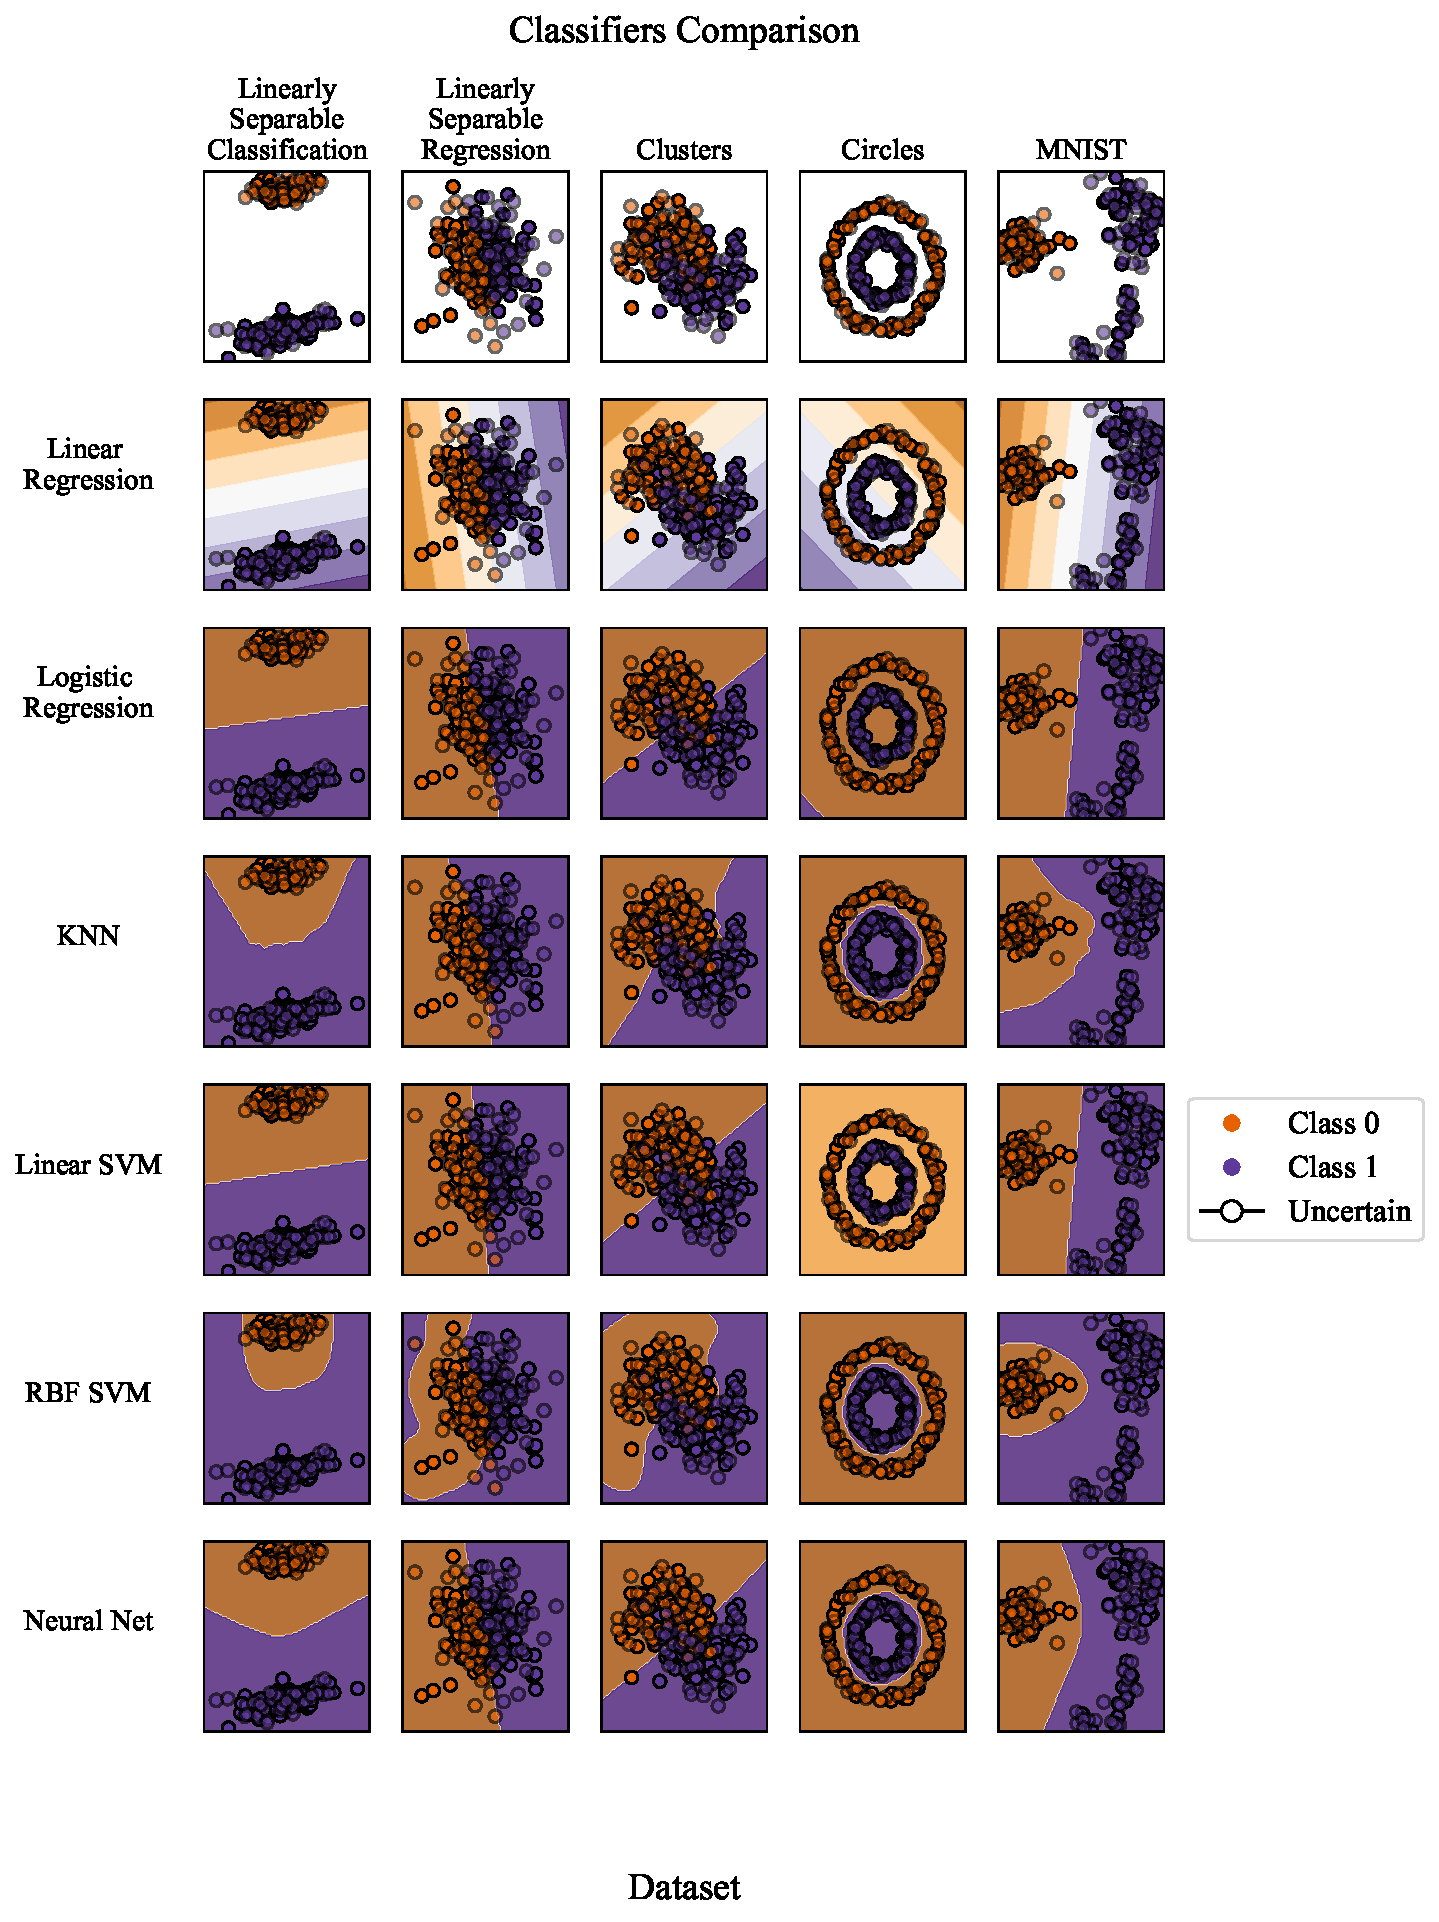
\includegraphics[width=.7\textheight, angle=90]{images/dataset_model_comparison.pdf}
    \caption{
    Each row depicts a different dataset where the values are classified into one of two classes, depicted by red or blue dots. 
    The model's \textit{decision boundary} is depicted using the red and blue gradients with darker colours corresponding to a more confident decision. 
    The first column depicts the raw input data and the true labels.
    Each other columns depicts the prediction using colour.
    The first 4 rows used generated two-dimensional data and the last row depicts a two-dimensional projection of the MNIST image dataset discussed in Section~\ref{subsec:methods-data} (since it would be impossible to plot the data in the 64 dimensions MNIST provides in the form of black and white pixels).
    }
    \label{fig:data_model_comparison}
    % \cm{todo: swap rows/columns, make full page, and update the caption accordingly}
\end{figure}


\section{Classical Methods}
Classical machine learning methods refer to models that rely on established statistical principles and typically make assumptions about the data structure. 
These models are often interpretable, computationally efficient, and serve as strong baselines for more complex approaches. 
Some of the most well-known classical methods include linear models, logistic regression, support vector classifiers (SVCs), and clustering algorithms like k-nearest neighbours (KNN).

\subsection{Parametric Models}
Parametric models are a class of models that summarize the data through a set of fixed parameters. 
These models assume a specific form for the underlying distribution of the data and require learning a finite number of parameters from the data. 
Once the parameters are estimated during model training, the model is fully defined, and predictions can be made.

\subsubsection{Linear Regression}
Linear regression is one of the simplest and most widely used models for supervised learning tasks. 
It models the relationship between a scalar dependent variable and one or more independent variables by fitting a linear equation to the observed data. 
However, there are certain disadvantages to this approach. 
Linear regression assumes that the relationship between the features and the target variable is, in fact, linear, which does not hold in many real-world scenarios.
See Figure~\ref{fig:data_model_comparison} to visualise the types of data that can be classified by this model.
Additionally, if the independent variables  are highly correlated, it may lead to multicollinearity, which can cause instability in the estimated parameters.
Despite its limitations, linear regression serves as a foundational model in machine learning, providing a solid basis for understanding more complex techniques.


\subsubsection{Logistic Regression}
Logistic regression is a widely used classification algorithm for binary outcomes, modelling the probability that a given input belongs to a particular class. 
Unlike linear regression, logistic regression uses a sigmoid (logistic) function to constrain the output between 0 and 1, making it ideal for probability estimation. 
Rather than producing an output that corresponds to a value in the range of  $(-\infty, +\infty)$ (as in the case of linear regression), it produces an output in the range $(0,1)$ which corresponds nicely with the notion of probability. 
In short, a logistic regression model produces an output that answers the question: ``what is the probability of an event when we assume a linear relationship between the input and the model weights?''


\subsubsection{Normality}

Throughout this thesis, data \textit{normalisation} is employed to standardise the columns of input data and assumes that the mean and standard deviation can be calculated from a sample of the true population.
Normalisation involves subtracting the mean from each sample and dividing by the standard deviation, resulting in values that represent the number of standard deviations each point lies from the mean. 
This transformation ensures comparability across features, even when their original scales differ significantly.

A key motivation for normalisation is to improve the numerical \textit{stability} of machine learning models. 
Normalised inputs reduce the risk of large output fluctuations in response to small input changes, thereby facilitating robustness.
The effectiveness of this process relies on the assumption that data is independently and identically distributed (i.i.d.). 
\textit{Independence} means that one observation does not influence another, while \textit{identically distributed} implies all samples originate from the same underlying distribution. 
These assumptions are foundational to many statistical methods.

Moreover, the Central Limit Theorem (CLT) supports the use of normalisation and normality-based techniques. 
It states that, for a sufficiently large sample size, the distribution of the sample mean approximates a normal distribution regardless of the original data distribution~\cite{stats}. 
In machine learning, this justifies the use of batch-wise statistics during training, as batch means tend to be normally distributed, enabling the application of methods that assume or benefit from normality~\cite{shalev2014understanding}.



\subsection{Non-Parametric Models}
Non-parametric models are a category of statistical models that do not assume a fixed number of parameters. 
Instead, they allow for greater flexibility in modelling complex datasets by letting the model structure grow with the data. 
This adaptability makes them particularly useful in situations where the underlying data distribution is unknown or highly variable. 
These models have no fixed assumptions about the underlying distribution of the data and some popular choices are outlined below. 

\subsubsection{KNN}
One non-parametric model used is $k$-nearest neighbours (k-NN), which is a type of instance-based learning where a data point is classified based on the majority class of its $k$ closest neighbours according to some relevant notion of distance. 
This model is widely used for classification tasks, and in Paper 5, it is specifically employed to cluster spam and non-spam internet traffic and content.

\subsubsection{Bootstrapping}

Another non-parametric model, called bootstrapping, is particularly useful for assessing the uncertainty or variability of an estimator without relying on strong parametric assumptions about the data's distribution. 
This method is used throughout the thesis to generate plots from the measured data, providing the uncertainty estimations that are denoted with error bars. 

\subsubsection{SVM}
Support Vector Machines (SVM) are a powerful class of supervised learning models used for classification and regression tasks. 
The core idea of SVM is to find a surface (often called a \textit{hyper-plane}) that best separates data points of different classes in a high-dimensional space.
While the basic SVM can be considered a parametric model (as it assumes that the data can be separated by a line), it becomes non-parametric when using kernel functions, which allow it to capture complex relationships in the data. 
This latter version is used in Papers II and V. 

These kernelised models are examined in greater detail in Papers II and  V. 
SVMs are effective when the number of features is much larger than the number of samples, which is common in text classification or biological data. 
This is also likely in the case of high resolution images as each megapixel of resolution yields 1 feature for each colour channel on each pixel-- meaning that 1 megapixel red/green/blue images correspond to 3 million features.

The use of kernel functions allows SVMs to perform well even when the data is not linearly separable by transforming the input into a higher-dimensional space.
Through kernel functions, SVMs can create complex, non-linear decision boundaries. 
Training an SVM can be slow, especially with large datasets, since it requires solving a quadratic programming problem~\cite{bottou2007support}.
The run-time of SVMs does not scale well with large datasets, both in terms of training time and memory requirements~\cite{bottou2007support}.
The decision boundary generated by SVMs, particularly with non-linear kernels, can be difficult to interpret~\cite{shalev2014understanding}.




\section{Neural Networks}
Neural networks are another class of ML models that can be both parametric~\cite{parametric_neural_network} and non-parametric~\cite{non_parametric_neural_network}. 
A neural network can be thought of as a graph composes of nodes that are connected by edges, composed of an input layer, one or more ``hidden'' layers that perform complex (non-linear) operations on the input data, and an output layer that returns a number, a vector of probabilities (called a \textit{soft label}), or a series of binary classifications (called a \textit{hard label}). 
Figure~\ref{fig:neural_network} depicts a simple neural network using circles to represent nodes, black lines to represent edges, and colour is used to identify input, hidden, and output layers. 

\begin{figure}[!ht]
\centering
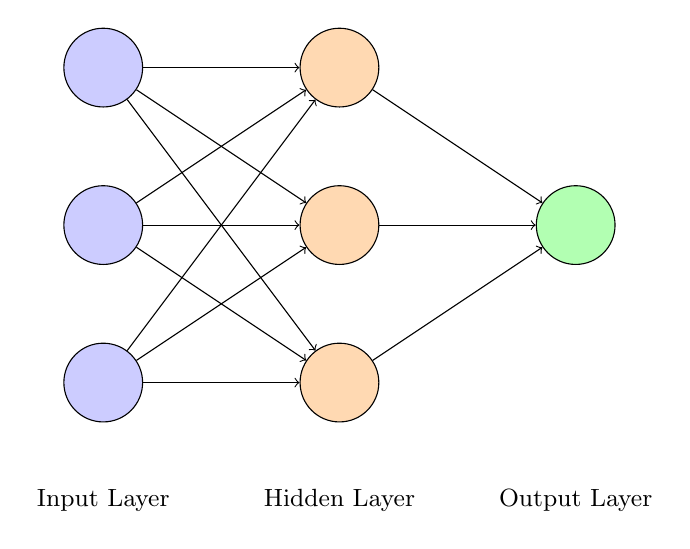
\begin{tikzpicture}[
    neuron/.style={circle, draw, minimum size=1cm},
    input neuron/.style={neuron, fill=blue!20},
    hidden neuron/.style={neuron, fill=orange!30},
    output neuron/.style={neuron, fill=green!30},
    layer/.style={draw=none, align=center},
    every node/.style={font=\small}
  ]

  % Input Layer
  \node[input neuron] (I-1) at (0,2) {};
  \node[input neuron] (I-2) at (0,0) {};
  \node[input neuron] (I-3) at (0,-2) {};
  \node[layer] at (0,-3.5) {Input Layer};

  % Hidden Layer
  \node[hidden neuron] (H-1) at (3,2) {};
  \node[hidden neuron] (H-2) at (3,0) {};
  \node[hidden neuron] (H-3) at (3,-2) {};
  \node[layer] at (3,-3.5) {Hidden Layer};

  % Output Layer
  \node[output neuron] (O-1) at (6,0) {};
  \node[layer] at (6,-3.5) {Output Layer};

  % Connections
  \foreach \i in {1,2,3}
    \foreach \h in {1,2,3}
      \draw[->] (I-\i) -- (H-\h);

  \foreach \h in {1,2,3}
    \draw[->] (H-\h) -- (O-1);

\end{tikzpicture}
\caption{A simple neural network with three layers. The input (blue), hidden (orange), and output (green) layers are colour-coded for clarity. The arrows indicate the flow of data.}
\label{fig:neural_network}
\end{figure}

Typically, state-of-the-art models are significantly more complex than the one pictured in Figure~\ref{fig:neural_network} and often rely on large numbers of hidden layers, complex structures (also called \textit{architectures}) that, for example, provide mechanisms to reinforce a certain behvaiour~\cite{reinforcement_learning} or enable time-dependent model configuration~\cite{lstm}.
Model architectures are sometimes chosen in an effort to model a particular biological~\cite{biomimicry_nn} or physical process~\cite{physics_nn}, though model architectures are often determined by brute-force trial and error~\cite{nn_architectures_brute_force}.

Regardless of the model architecture, training a neural network requires the definition of a loss function—a quantitative measure of how far the model’s output deviates from the expected result. 
The choice of loss function is often dictated by the task at hand: for example, cross-entropy loss is widely used for classification problems~\cite{shalev2014understanding} because it naturally penalizes confident but incorrect predictions; whereas mean squared error~(MSE)~\cite{stats} is commonly applied in regression tasks where the goal is to minimize the average squared difference between predicted and actual values. 
More sophisticated loss functions can encode domain-specific requirements, such as robustness to outliers~\cite{zhang2015outlier}, uncertainty visualisation~\cite{model_uncertainty}, or fairness constraints~\cite{mehrabi2021survey}, and can be custom-designed to reflect complex trade-offs or safety margins.

The optimization process involves adjusting the network’s internal parameters—typically millions or even billions of weights and biases—to minimize the chosen loss function across a given dataset. 
This is most often done using stochastic gradient descent (SGD) or one of its many variants (e.g., Adam~\cite{adam}, RMSProp~\cite{rmsprop}, or Adadelta~\cite{adadelta}) which iteratively updates model parameters in the direction that minimises the chosen loss function by comparing model predictions to the ground truth.

The optimization landscape of a deep neural network is highly non-convex--- it often contains numerous local minima, saddle points, and flat regions. 
In practice, modern optimization algorithms, combined with techniques like learning rate scheduling~\cite{learning_rate_scheduling}, regularization~\cite{xu2009robustness,jakubovitz2018improving,ross2018improving}, momentum~\cite{momentum}, and batch normalization~\cite{batch_normalisation}, enable effective navigation of this complex terrain. 
However, convergence to a low loss value does not necessarily imply generalisation to new data.
As a result, the optimization process is closely tied to  the choice in validation metric~\cite{carlini2019evaluating} and techniques for measuring generalisation error like cross-validation scoring~\cite{shalev2014understanding} are used to ensure that the network not only performs well on training data but also works well \textit{in general}.

Furthermore, in domains such as healthcare, aviation, or autonomous systems, loss functions and optimization criteria may be carefully designed to reflect asymmetric costs of error~\cite{meyers2023safety}. 
For instance, this might mean penalizing false negatives more heavily than false positives when a missed detection could result in harm than a false positive. 
In other cases, this might mean providing mechanisms to notifying a user when a given classification is uncertain~\cite{model_uncertainty}.
This further reinforces the idea that model training is not merely a numerical process, but a design decision that must align with the broader goals of safety, reliability, and ethical deployment.
Nevertheless, even an excellent score on well chosen metric does not guarantee legally compliant performance in the presence of an adversary~\cite{meyers2023safety,meyers2024massively,trashfire,meyers_aft}, which are characterised further in Chapter 4. 
For now, suffice it to say that not only do the regulatory concerns outlined in Chapter 2 remain persistent threats to large-scale machine learning methods, but that they raise serious ethical concerns more broadly.

\section{The Ethics of ML}
\label{sec:ethics}
The problems with the typical approach to ML are numerous. 
Recently, marginal gains in accuracy have relied on increasingly larger models to produce marginal gains~\cite{desislavov2021compute}. 
These models rely on massive datasets~\cite{desislavov2021compute,vapnik1994measuring,blumer1989learnability}, from an ever-shrinking number of sources~\cite{koch2021reduced}, leading to gender-biased models~\cite{lu2020gender}, race-biased models~\cite{buolamwini2018gender}, and critical design errors~\cite{banks2018driver}. 
This trend isn't new and goes back decades~\cite{corsaro1982something,ramirez2000resource,buolamwini2018gender}. 
Despite this, it has been suggested that large scale ML methods be used to detect (\textit{potentially}) illegal material~\cite{abelson2021bugs}.
Since client-side monitoring with neural networks was recently the subject of a proposal by the EU parliament to stop the spread of offensive and harmful online contact, it can be used as a simple case study in how \textit{obviously} ``good'' models have inherent risks.
One, these models are not nearly reliable enough to be deployed in situations that can negatively effect a human, which is detailed in the previous chapter. 
Second, these models can reveal the private data used to train the model~\cite{extraction_attack} or used to generate novel content that is similar to restricted images~\cite{deepface_attack}.
Third, these models are inherently biased--- relying on statistical assumptions that harm already marginalised groups \cite{buolamwini2018gender}. 
Fourth, the existence of the model comes with unforeseen environmental and societal costs-- potentially chilling dissent or speech~\cite{abelson2021bugs}, using immense computational resources~\cite{ai_power}, and outsourcing of the data labelling to low wage workers who have to view the offensive content~\cite{ai_inequity}.
Finally, modern ML systems in general have questionable reliability on edge cases, but nevertheless induce real experts to misjudge the quality of the model output~\cite{chatgptlawyer,teslasleep1,teslasleep2,teslasleep3,perry2023users,rosenbacke2024ai}.
In short, there are many ethical questions to consider when deploying an ML model which have been clustered into efficacy, privacy, security, reliability, and the environment.  
In the following,  




\subsection{Reliability}
\label{subsec:reliability}
Fundamentally, ML systems are just statistical models that have the the ability to over-generalise.
ML models have shown themselves capable of performing exceptionally well on a wide variety of tasks. 
For example, there are thousands of papers that report
However, much research has also noted the fragility of these models to small changes in the input space. 
One particular concerning example is the inability of state-of-the-art image classification systems to handle data that comes from a different distribution than the training set~\cite{bungert2023understanding}. 
One proposed source of this error is ``hidden stratification''--- the unknown subsets of the data that are unaccounted for in the model~\cite{hidden_stratification}.
Another often-discussed source of unreliability is the ``long-tail problem'' that describes the problem of the wide distribution of real-world cases outside of the ``normal'' distribution learned from the training set.
This 2021 survey of wildlife identification models examined methods for mitigating the effect of these out-of-distribution new samples and their best attempt still confidently returned an incorrect answer nearly 30\% of the time.
Another author notes that the standard model output layers do not even return meaningful confidence intervals~\cite{medical_failure_detection}.
Some authors \cite{birhane2021algorithmic} recommend a set of ethics that centres machine learning research on groups mostly likely to be adversely effected. 
However, since these groups tend to be marginalised or statistical outliers compared to dominant groups, there's an inherent tension within this recommendation. 
Let's take the case of the autonomous (self-driving) car. On one hand, we would like cars to not mistake women, minority groups, or gender non-conforming people for inanimate objects. 
On the other hand, the statistical variance introduced by these statistically less ``normal'' subsets of people will cause a degradation of performance for the ``average'' user. 
Is it more fair to reduce the accuracy overall for the sake of statistically ``abnormal'' groups rather than maximise the performance on the statistically average person? 
This tension was proven to be inherent to the statistical methods underlying machine learning systems \cite{carlini_towards_2017}. 
This tension is widely discussed in the literature on fairness for machine learning as well~\cite{feuerriegel2020fair,van2021fairness,corbett2018measure}. 
To be clear, this isn't a problem that is restricted to discrete classes like skin colour or apparent gender, but is can be extended to any statistically ``abnormal'' situation.
While some mitigation strategies have been proposed~\cite{medical_failure_detection,medical_ML_methodology}
The intention here is not to single-out medical imaging as a potentially risky application of ML as industrial control~\cite{ai_industry} software, aviation control software~\cite{ai_aviation}, autonomous cars~\cite{ai_automotive}, bank loaning algorithms~\cite{ai_finance}, criminal justice administration tools~\cite{ai_prison}, predictive policing algorithms~\cite{ai_security}, home pricing algorithms~\cite{ai_home_pricing}, and computer-vision based security checkpoints~\cite{ai_luggage} are built from the same models.


\subsubsection{Reproducibility}
\label{subsec:reproducibility}

Unlike the experiments detailed in the included papers, ML research models are typically not reproducible. 
Firstly, there is a problem of scale as ML research has increasingly shifted to industry due to the massive costs associated with training state-of-the-art models~\cite{ai_cost_comparison}. 
This is in no small part due to the scale of both modern models and their associated datasets~\cite{desislavov2021compute,ai_power} which have grown in size~\cite{desislavov2021compute} and increasingly come from fewer sources~\cite{koch2021reduced}. 
For example, commercially deployed image recognition systems~and large-language models can cost millions of dollars of compute time to train~\cite{ai_cost_comparison}, making reproducing state-of-the-art research infeasible under the current peer review system. 
Even when model architectures are fully released, critical components can be omitted or under-specified---including details about training schedules, hyper-parameter selection, hardware or network configuration, and random seed initialisation~\cite{medical_reproducibility}.
Furthermore, proprietary models are never released at all and the training data remains entirely private, creating a performance gap between academic benchmarks and real-world implementations~\cite{croce_reliable_2020}. 
Without verifiable and consistent performance it is impossible to determine efficacy or establish accountability.
Reproducibility is a prerequisite for trustworthy, reliable ML systems and dataset and pipeline transparency have recently become the subject of regulatory concern~\cite{ai_pipeline_regulation}. 
Another critical dimension of reliability in machine learning systems is the presence and persistence of bias. While reproducibility ensures consistency across deployments, it does not guarantee fairness or equity in a model’s predictions. 
A perfectly reproducible model can still systematically disadvantage certain groups if it reflects biases present in the training data or embedded in its design choices~\cite{buolamwini2018gender,raji2019actionable,lu2020gender}. 
This is especially dangerous in safety-critical applications, where biased outcomes can have life-altering consequences which would be disproportionately felt by statistically marginal groups.

\subsubsection{Bias}
\label{subsec:bias}
ML systems are subject to the same biases as their human creators and their datasets. 
For example, gender-biased modelling leads to significantly higher fatality in car accidents for female-bodied people~\cite{evans2001gender}. 
In another instance, researchers found neural networks that unintentionally encode racial information from medical imaging data that should not encode such information~\cite{gichoya2022ai}. 
Nevertheless, the problems are not intractable. 
Since these models mathematically agnostic, the problems and solutions are strictly human. 
After raising awareness about the racial- and gender discrepancies in facial recognition systems \cite{buolamwini2018gender}, subsequent research found that the problem was substantially reduced \cite{raji2019actionable}, perhaps with nothing more than changing the sampling method. 
However, computer science as a whole has struggled with racial and gender biases during hiring process already exist \cite{rattan2019identical,yarger2020algorithmic} and other research examines how this permeates across the field of machine learning \cite{birhane2021algorithmic}.

Let's take the case of the autonomous (self-driving) car.
On one hand, we would like our car to not mistake women, minority groups, or gender non-conforming people for inanimate objects. 
On the other hand, the statistical variance introduced by these statistically less ``normal'' subsets of people will cause a degradation of performance for the ``average'' user. 
Is it more fair to reduce the accuracy overall for the sake of statistically ``abnormal'' groups rather than maximize the performance on the statistically average person? 
This tension is widely discussed in the literature on fairness for machine learning as well~\cite{feuerriegel2020fair,van2021fairness,corbett2018measure}. 
The goal then, must be, to meet the legal definitions of safe in \textit{all} cases, which inherently means considering the worst-case counter-examples, edge cases, and statistical margins.
For all classification models, it has been shown that these misclassifications are inherent to the task of categorisation~\cite{dohmatob_generalized_2019}.
Nevertheless, because these models \textit{seem} to be performing human-like tasks, these systems induce problematic levels of trust.

\subsection{Deferred Expertise}
\label{subsec:false_expertise}
Because systems like ChatGPT or Tesla's self-driving software \textit{appear} to have human levels of intelligence, it is not uncommon for users to trust these systems more than they should. 
Despite the infancy of the technology, complicated machine learning software has  already fooled users into complacency. 
There are no shortage of examples of drivers falling asleep while operating Tesla cars in ``full self-driving'' mode, sometimes leading to fatal driving accidents~\cite{teslasleep1,teslasleep2,teslasleep3}. 
Lawyers have faced penalties for inappropriate usage of chatbots wherein case law was invented wholesale by models not designed to produce accurate text~\cite{chatgptlawyer}.
One study showed that individuals who use ML-based code assistance not only trusted their code more, but were also more likely to produce code with security flaws~\cite{perry2023users}. 
Another study showed that the accuracy of medical diagnoses is expected to decrease between 5-30\% with the introduction of ML-based assistance for medical doctors due to false confirmation errors~\cite{rosenbacke2024ai}. 

These issues of misplaced trust and over-reliance on machine learning systems underscore a broader point: ML models, while powerful, are not autonomous experts. 
Their perceived authority often exceeds their actual capability, introducing new risks and compounding existing ones~\cite{chatgptlawyer,perry2023users,rosenbacke2024ai}. 
However, the implications of widespread machine learning adoption extend beyond human trust and safety. 
Even when model make their users fully aware of their limitations, the models come with substantial environmental costs~\cite{ai_environment}. 



\subsection{Environmental Concerns}
The development, training, and deployment of modern machine learning models demand enormous computational and data resources, which in turn translate to high energy consumption~\cite{ai_power}, hardware waste~\cite{ai_environment}, and broader sustainability challenges~\cite{ai_water,indian_point}.
Furthermore, data collection can be very costly~\cite{roh2019survey}, increases development time~\cite{lam2004new}, and makes it harder to verify a product~\cite{zirger1996effect}. 
\label{subsec:environment}

As machine learning systems continue to scale in complexity and deployment, their environmental impact has become a growing concern among researchers, policymakers, and practitioners. 
While the societal benefits of ML are allegedly significant, they come at a substantial ecological cost that is often under-reported and poorly accounted for in system evaluations.

Training state-of-the-art models—particularly large language models and computer vision systems—requires enormous computational resources~\cite{ai_power}. 
These training runs can span days or weeks across thousands of high-performance GPUs, consuming megawatt-hours of electricity and contributing significantly to carbon emissions~\cite{strubell2020energy}. 
For example, the training of a single large-scale language model has been estimated to emit as much carbon as five average American cars over their entire lifetimes~\cite{strubell2020energy}. 
As models become larger and more capable, their environmental footprint continues to grow unless mitigated by advances in hardware efficiency, algorithmic optimization, or the adoption of green energy sources.

Beyond training and inference, environmental costs accrue throughout the ML lifecycle. Data collection is not only time-consuming and labour-intensive~\cite{roh2019survey}, but also energy-intensive—--particularly when involving data-intensive processes like web scraping, sensor networks, or other real-time data pipelines~\cite{ai_power}. 
Preprocessing and cleaning this data can further increase compute overhead, extending development cycles~\cite{lam2004new} and complicating verification procedures~\cite{zirger1996effect}. 
Moreover, the continual deployment and fine-tuning of models in production environments adds to long-term infrastructure demands, especially in cases where retraining is frequent or large models are frequently synchronised across a network.

Hardware production for ML also presents a growing sustainability issue. 
The demand for GPUs and specialized accelerators has led to increased extraction of rare earth metals and non-renewable materials~\cite{ai_environment}. 
This contributes to electronic waste and accelerates hardware obsolescence as newer, more powerful chips are released to support ever-larger models~\cite{desislavov2021compute}.

These challenges have prompted early efforts to promote sustainable machine learning. 
Some proposals include carbon-aware scheduling of training jobs~\cite{anthony2020carbontracker}, algorithmic innovations like sparse training and pruning~\cite{islam2024sustainable}, and better reporting standards that include metrics like energy usage and emissions alongside traditional performance scores~\cite{anthony2020carbontracker}.

As machine learning continues to be deployed in safety-critical domains, it is vital that environmental sustainability becomes a core consideration—just as safety, security, privacy, and reliability are. 
Ignoring these costs risks creating systems that may be technically impressive but environmentally unsustainable at scale and further exacerbate global inequities around who benefits from the deployment of these models.

While Chapter 2 outlined the regulatory and safety challenges surrounding machine learning, and this chapter has explored the structural and ethical dimensions of model development, it is crucial to recognize that even well-intentioned, well-designed, and well-regulated systems can be actively subverted—--an increasingly urgent concern addressed in next chapter.

\include{ch_4_adversaries}

\chapter{Verification and Validation}
\label{ch:vnv}
The previous chapters introduced the ML pipeline, outlined the regulations that govern safety and privacy, examined some particular ML models, and described a very real threat model against them in the form of attacks. 
In contrast, this chapter discusses the ways in which this thesis adheres to and promotes best practices for reproducibility and auditability.
Verification and validation (V\&V) broadly refers to the processes used to ensure that a system meets its requirements and behaves safely and reliably under expected-- and unexpected-- conditions.
V\&V methods can broadly be classified into several categories: formal verification, simulation, empirical modelling, and static or dynamic analysis.
Fields like aviation, automotive, and medicine use some combination of these to mitigate and control risks on a daily basis.


\section{Formal Verification}
Formal verification is a method of mathematically proving the correctness of a system with respect to a formal specification. 
Unlike simulation, which tests a system under selected scenarios, formal verification attempts to exhaustively prove that certain properties (\textit{e.g.}, safety, robustness, or correctness) always hold, regardless of the input or system state. 
This makes it especially attractive in systems where failure is catastrophic and exhaustive testing is infeasible.

The strength of formal verification lies in its guarantees: if a property is proven, it holds for all cases within the bounds of the assumptions made. 
However, this rigour comes with significant costs and complexity. 
Creating formal specifications requires a precise and often abstract understanding of the system, and the proofs themselves can be highly non-trivial, requiring expert knowledge and substantial computational resources~\cite{formal_adversarial,vehicle_formal}.

An important example of formal verification is the CompCert C compiler, which has been formally verified to produce assembly code that is functionally equivalent to its source code~\cite{leroy2009formally}. 
In contrast to conventional compilers, which may contain bugs in optimisation or code generation, CompCert offers mathematical guarantees of correctness, making it appealing for critical systems such as avionics and medical devices.
In medical devices, formal verification has been applied to implantable cardiac pacemakers, which must maintain life-critical timing constraints to not accidentally kill the person they are meant to help.
Research efforts, such as those of Jiang et al.~\cite{jiang2012modeling}, have demonstrated how formal models of pacemaker logic can be verified to ensure that the device will never enter dangerous states, even under extreme timing conditions or unexpected cardiac rhythms.

In the domain of machine learning, formal verification is becoming increasingly relevant, as ML models are being deployed in safety-critical applications such as autonomous vehicles, medical diagnostics, and security systems. 
Verifying the correctness of ML models with respect to a formal specification presents unique challenges compared to traditional software systems. Unlike conventional software, ML models are typically data-driven and may exhibit unpredictable behaviour due to the complex nature of their learned representations. 
Despite these challenges, researchers have developed techniques for formal verification of certain aspects of ML models, such as ensuring robustness to adversarial attacks or proving the correctness of a model’s decision-making process in specific environments. 
While the field is still in its infancy, work has been done in verifying neural networks' robustness to adversarial perturbations and ensuring that certain fairness constraints are met during the learning process~\cite{formal_adversarial}.
However, these formal methods can be computationally infeasible or altogether useless during model selection~\cite{vehicle_testing_review}.

As ML models continue to play a larger role in critical applications, the need for formal verification to guarantee their reliability and safety will only grow.
While formal verification guarantees the correctness of a system through mathematical proofs, simulation provides a way to find how common error states and other extreme conditions are.


\section{Simulation}
Simulation is a powerful verification technique in which complex systems are modelled and tested under a variety of conditions before real-world deployment. These techniques are especially prominent in high-stakes domains such as aerospace, automotive safety, and medical science, where real-world testing is expensive, dangerous, or ethically challenging.

In the aerospace industry, simulation is integral to the development and certification of an aircraft. 
One well-known example is the Boeing 777, which was the first commercial aircraft to be entirely designed using computer-aided design (CAD) and simulation tools, minimising the need for physical prototypes~\cite{boeing777}.
It is also famous for being the first ``fly-by-wire'' system where manual pilot input was replaced with electrical signals and onboard computers which forced the industry to simulate physical interactions in software to ensure safety~\cite{boeing777}.

In automotive engineering, crash simulations are widely used to complement physical crash testing. 
However, these simulations often rely on models based on the median male body, leading to safety designs that disproportionately protect average-sised men. Research has shown that women are significantly more likely to suffer injury in car crashes due to this bias in crash test dummies and the resulting simulations~\cite{crashgenderbias}.

Similarly, in medical science, simulations of drug interactions or disease progression are often built from datasets that over-represent male physiology~\cite{merone2022sex}. 
This has led to a ``male body problem'' in medical research, where treatments may be less effective or riskier for women. 
Additionally, statistical analyses in clinical trials often rely heavily on p-values, which can misrepresent the reliability of results when not properly contextualised---known as the p-value problem~\cite{goodman1993p}.

Unlike physical systems that are governed by well-known physical laws, many ML models can be hard to explain or interpret~\cite{explainable}. 
By harnessing adversarial attacks to simulate worst-case samples, model builders can test the robustness and reliability of machine learning systems under extreme or intentionally challenging conditions.
Adversarial simulation involves creating perturbed inputs that are specifically designed to cause model failures, revealing vulnerabilities that may not appear under standard testing conditions~\cite{fgm}.
This approach enables practitioners to stress-test models systematically before they are deployed in the real-world. 
However, there is a data-driven approach that relies on real-world experimentation call.

\section{Empirical Modelling}

Empirical models can take various forms, such as statistical models, ML models (Chapter 3), or system dynamics models (\textit{e.g.} structural or mechanical engineering~\cite{structural_eng}). 
For example, a simple statistical model is the exponential distribution, which is often applied in reliability engineering to model the time between events in systems that experience a constant failure rate over time.
A classic example from reliability engineering is the exponential distribution, which models the time between failures in systems that exhibit a constant failure rate. 
This distribution is defined by a single parameter, $\lambda$, the rate of failure (or the inverse of the mean time between failures). 
Its probability density function (PDF) is:

\begin{equation*} f(t) = \lambda e^{-\lambda t} \quad \text{for } t \geq 0, \end{equation*}

where $f(t)$ denotes the likelihood of failure at time $t$. 
While analytically simple, this model assumes a constant hazard rate, which is often unrealistic for complex systems.

More flexible are survival models, which do not assume a constant failure rate and are therefore better suited for modelling the complex relationship between times, cost, and robustness.
These models are explored in detail in Paper~III, where survival time is used as a proxy for model robustness, and in Paper~IV, which employs accelerated failure time (AFT) models to analyse adversarial robustness across neural networks trained on different hardware architectures.

In an AFT model, the log of survival time is modelled as a linear function of covariates:

\begin{equation*} 
\log(T) = \beta_0 + \beta_1 x_1 + \beta_2 x_2 + \cdots + \beta_k x_k + \varepsilon, \end{equation*}

where $T$ is the survival time, $x_i$ are covariates (e.g., model depth, learning rate, hardware type), $\beta_i$ are model coefficients, and $\varepsilon$ is a random error term. This allows interpretation of covariates as multiplicative effects on the survival time, offering a more intuitive understanding of robustness under adversarial pressure.

Survival models play a critical role across a range of domains where understanding time-to-event behaviour is essential. 
In medicine, survival analysis is extensively used in epidemiological studies to model patient survival times, time until disease recurrence, or time to recovery~\cite{aft_models}. 
In medicine, covariates such as age, treatment type, genetic markers, and co-morbidities are incorporated to estimate patient-specific risks and guide personalised treatment strategies~\cite{aft_models}. 
In the automotive domain, survival models help assess the reliability and durability of components, such as engines, brake systems, and electrical subsystems. 
By analysing failure times under different usage conditions and environments, manufacturers can improve design, schedule preventive maintenance, and optimise warranty policies~\cite{automotive_survival}. 
In aircraft design, survival analysis informs the estimation of failure probabilities for critical components under stress, load, and fatigue over time~\cite{aircraft_survival}. 
These models support decisions in structural engineering, maintenance scheduling, and certification by regulatory authorities to ensure high standards of safety and reliability throughout the aircraft’s operational lifecycle~\cite{aircraft_survival}.


\section{Static and Dynamic Analysis}

When building a bridge, static analyses are used to estimate the forces acting on a component when a part is not moving and dynamic analyses are used to estimate forces when acceleration is experienced~\cite{structural_eng}.
This same metaphor can be applied to software development---where static analysis examines code for errors, vulnerabilities, and compliance issues without executing it~\cite{beller2016analyzing}, while dynamic analysis tests and monitors the software during runtime to uncover defects that only appear during execution~\cite{ball1999concept}. 
These two approaches were applied throughout this thesis to ensure the correctness, reliability, and reproducibility of the developed software and experimental results.

In automotive or aviation, physical components such as engines, control surfaces, or braking systems are subjected to both static and dynamic analyses to verify their integrity under both constant and changing loads. Similarly, embedded software controlling these components undergoes static analysis to catch coding errors early and dynamic analysis to validate behaviour under real-world operational conditions~\cite{boeing777}.
In medical or banking software, static analysis is critical to ensure compliance with regulatory standards like HIPAA or GDPR by identifying security vulnerabilities and logical errors before deployment, while dynamic analysis is employed to validate the correctness, reliability, and security of live systems handling sensitive patient or financial data~\cite{jetley2008static,kuncoro2017mobile}.

Throughout this thesis, static analyses in the form of pre-commit scripts~\cite{precommit} and unit tests~\cite{testautomation} were used to ensure code quality, consistency, and the early detection of potential errors before code was used for experimentation as well as in the generation of the included papers. 
Pre-commit hooks are automated scripts that run a set of checks---such as linting, formatting enforcement, or static code analysis---each time a developer attempts to make a change to the source code, effectively acting as a gatekeeper to prevent problematic code from entering the codebase~\cite{precommit}.
All papers were formatted for consistency in this way and all source code was evaluated for things like unreachable code, undeclared variables, and un-tested functions.
In addition, functional and integration tests were used to conduct dynamic analyses of the software components developed. 
Functional tests verify that individual functions or features perform as expected when executed and integration tests, on the other hand, validate that different modules or services interact correctly and robustly when combined, ensuring that defects that only emerge from complex system interactions are detected and addressed during runtime~\cite{wang2006software}.
Furthermore, each paper and the source code for the experiments has been made available as part of the software package described in Paper VI thus ensuring that anyone can verify and validate the findings presented in this thesis. 

\section{Accuracy is Not Enough}

As we move from modelling individual components to reasoning about system-level reliability, a more fundamental question arises: ``how can we trust complex systems whose behaviours are shaped by large-scale, opaque, and data-dependent models?''

Historically, marginal gains in model performance have come at the cost of exponentially larger models~\cite{desislavov2021compute}. 
Large models require increasingly vast datasets~\cite{desislavov2021compute,vapnik1994measuring,blumer1989learnability}, which are collected, catalogued, distributed by narrowing number of elite and well-funded institutions~\cite{koch2021reduced}. 
By amplifying systematic biases, this concentration introduces critical risks, including gender bias~\cite{lu2020gender}, racial discrimination~\cite{buolamwini2018gender}, and fatal design flaws~\cite{banks2018driver}. 
These concerns are not new~\cite{corsaro1982something, ramirez2000resource, buolamwini2018gender}; they echo through decades of evidence showing higher fatality rates for female-bodied individuals in car accidents~\cite{evans2001gender}, or neural networks that inadvertently encode racial information from medical images ~\cite{gichoya2022ai}.

Beyond social and ethical implications, data collection and labelling for machine learning itself introduces a host of practical concerns. 
It is expensive~\cite{roh2019survey}, raises significant privacy issues~\cite{bloom2017self}, extends time-to-market~\cite{lam2004new}, slows innovation~\cite{zirger1996effect}, and relies on vast numbers of outsourced workers~\cite{ai_inequity}.
Worse still, performance metrics in machine learning often paint an overly optimistic picture~\cite{madry2017towards,croce2020reliable}. 
As researchers have noted~\cite{madry2017towards,carlini_towards_2017,croce_reliable_2020,meyers}, traditional test/train evaluation only uncovers failures within the training distribution which leaves models vulnerable to catastrophic failures when deployed in the real world.

To build truly trustworthy systems, model builders must go beyond conventional benchmarks and provide strong, actionable guarantees. 
These guarantees must address the practical, social, and technical limitations outlined above--—and they must do so efficiently. 
In particular, we need rigorous, cost-effective methods for verifying model behaviour under diverse and challenging conditions, ideally fast enough to be integrated into development feedback loops and used in simulation, rather than relying on deployment in real-world systems like autonomous vehicles, delivery drones, or manufacturing robots.

Papers I and II examines the run-time and efficacy of several adversarial attacks and model defences in an effort to find which defences are trustworthy.
Paper III presents a metric for quantifying the trust of a model against a given set of attacks and Paper IV uses this to build models that are not only more trustworthy, but also more power and cost efficient. 
Paper V then outlines a model that aims to keep user data private and thus be more trustworthy by default. 
Finally, Paper VI outlines a safety-critical framework for ML verification and validation and presents the software tooling required to not only reproduce the work included in this thesis, but to conduct the same type of massive and rigorous evaluations of any ML model trained on any dataset.

\include{ch_6_summary_of_contributions}

\printbibliography
\cleardoublepage


% ------------------------------------------------------
%  The papers
% ------------------------------------------------------
% Commented these out to reduce render time
% \clearpage\mbox{}\clearpage %%USE IF ODD NUMBER OF PAGES IN INTRO
\thispagestyle{empty}
\raisebox{-30 mm }{
  \makebox[21cm]{
    \raggedleft                       
    \fontsize{24.88}{30} \bfseries Paper
    \colorbox{black}{
      \framebox[3cm][l]{
        \color{white}{\null\hspace{-3pt}I}
        \rule[-8pt]{0pt}{36pt}        
      }
    }
  }
}
\vspace{-7pt}

\noindent
\rule[1mm]{412pt}{2pt}
\\{}\\ 
\phantomsection
\label{paper_one}
\PaperI
\addcontentsline{toc}{chapter}{Paper I}
\clearpage\mbox{}\thispagestyle{empty}\clearpage
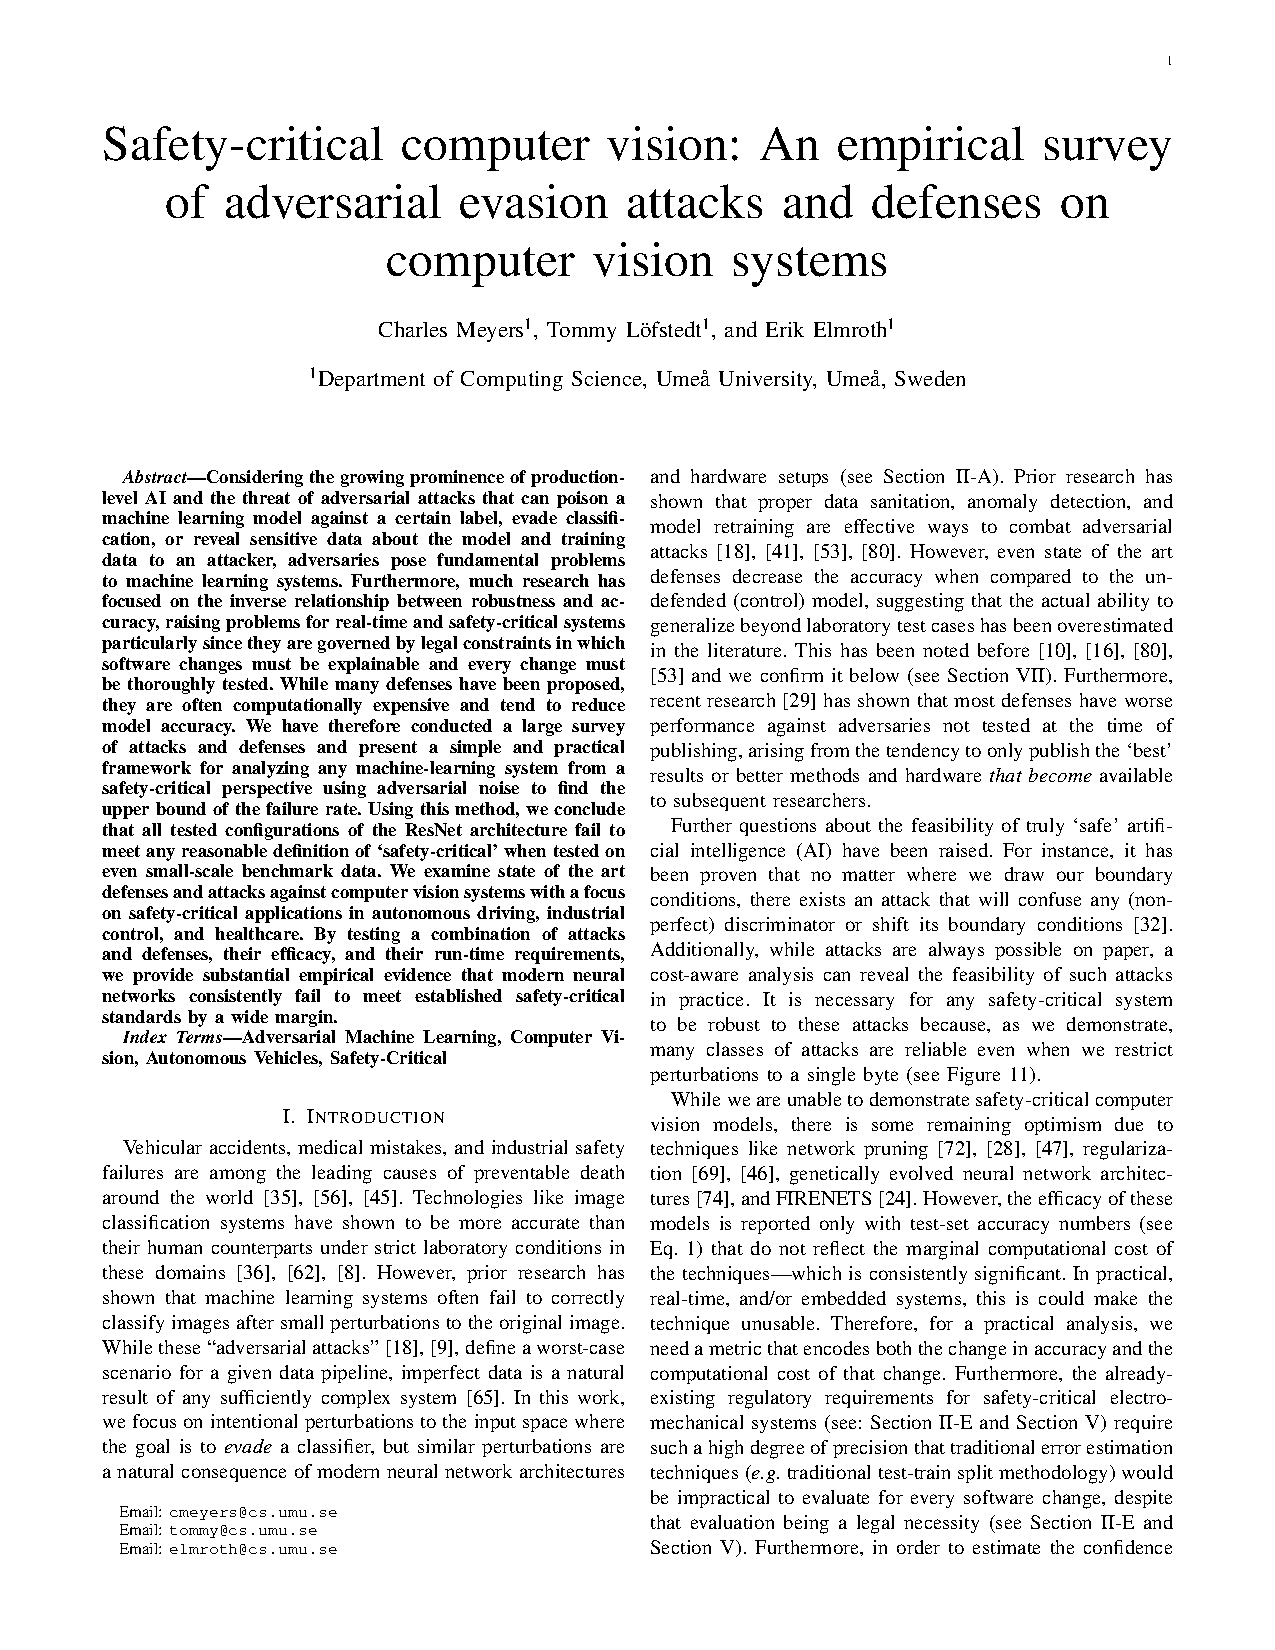
\includepdf[pages=-]{papers/Paper1.pdf}
\clearpage


%\clearpage\mbox{}\clearpage %%EMAD USE IF ODD NUMBER OF PAGES PRECEDING
\thispagestyle{empty}
\raisebox{-30 mm }{
  \makebox[21cm]{
    \raggedleft                       
    \fontsize{24.88}{30} \bfseries Paper
    \colorbox{black}{
      \framebox[3cm][l]{
        \color{white}{\null\hspace{-3pt}II}
        \rule[-8pt]{0pt}{36pt}        
      }
    }
  }
}
\vspace{-7pt}

\noindent
\rule[1mm]{412pt}{2pt}
\\{}\\ 
\PaperII
\addcontentsline{toc}{chapter}{Paper II}
\clearpage\mbox{}\thispagestyle{empty}\clearpage
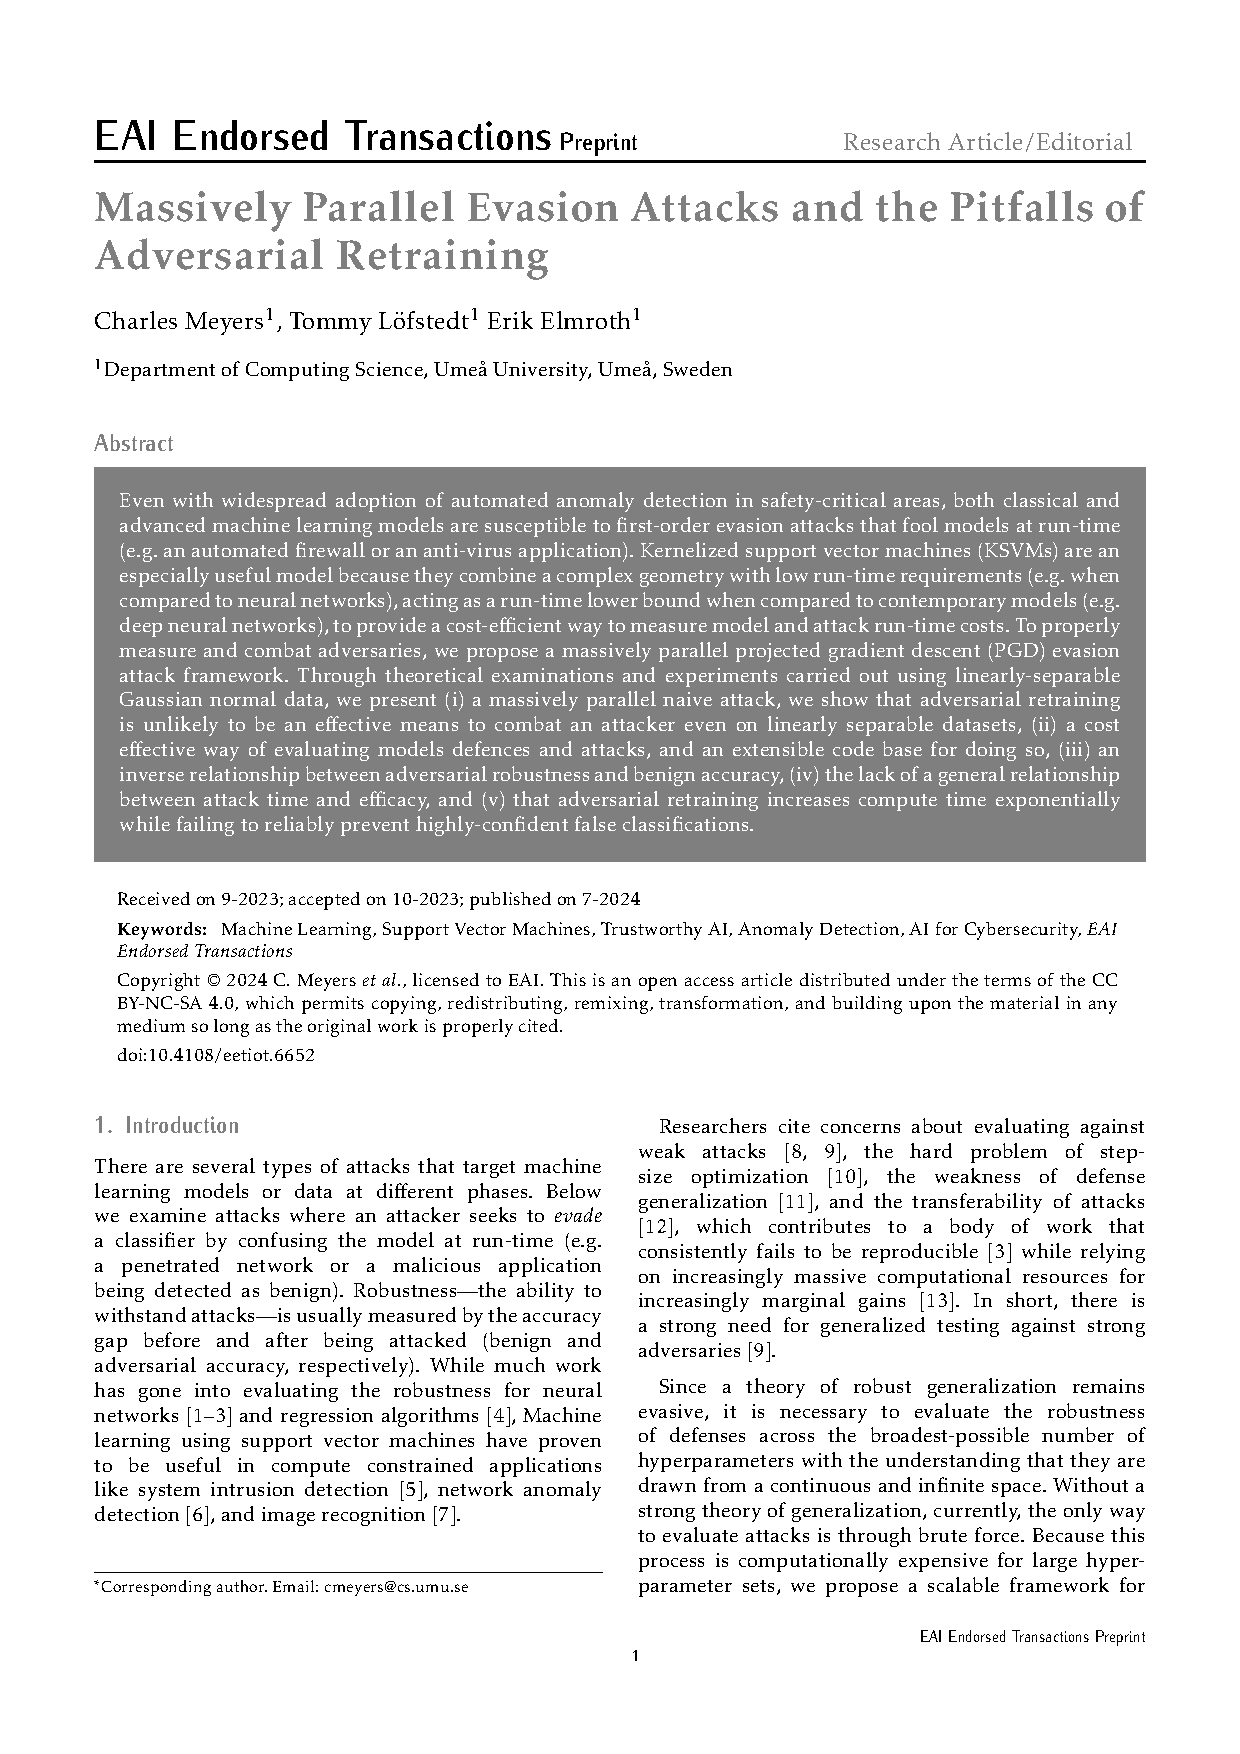
\includepdf[pages=-, pagecommand={}]{papers/Paper2.pdf}
\clearpage
\input{papers/paper3}
\input{papers/paper4}
%\clearpage\mbox{}\clearpage %%EMAD USE IF ODD NUMBER OF PAGES IN INTRO
\thispagestyle{empty}
\raisebox{-30 mm }{
  \makebox[21cm]{
    \raggedleft                       
    \fontsize{24.88}{30} \bfseries Paper
    \colorbox{black}{
      \framebox[3cm][l]{
        \color{white}{\null\hspace{-3pt}V}
        \rule[-8pt]{0pt}{36pt}        
      }
    }
  }
}
\vspace{-7pt}

\noindent
\rule[1mm]{412pt}{2pt}
\\{}\\ 
\PaperV
\addcontentsline{toc}{chapter}{Paper V}
\clearpage\mbox{}\thispagestyle{empty}\clearpage
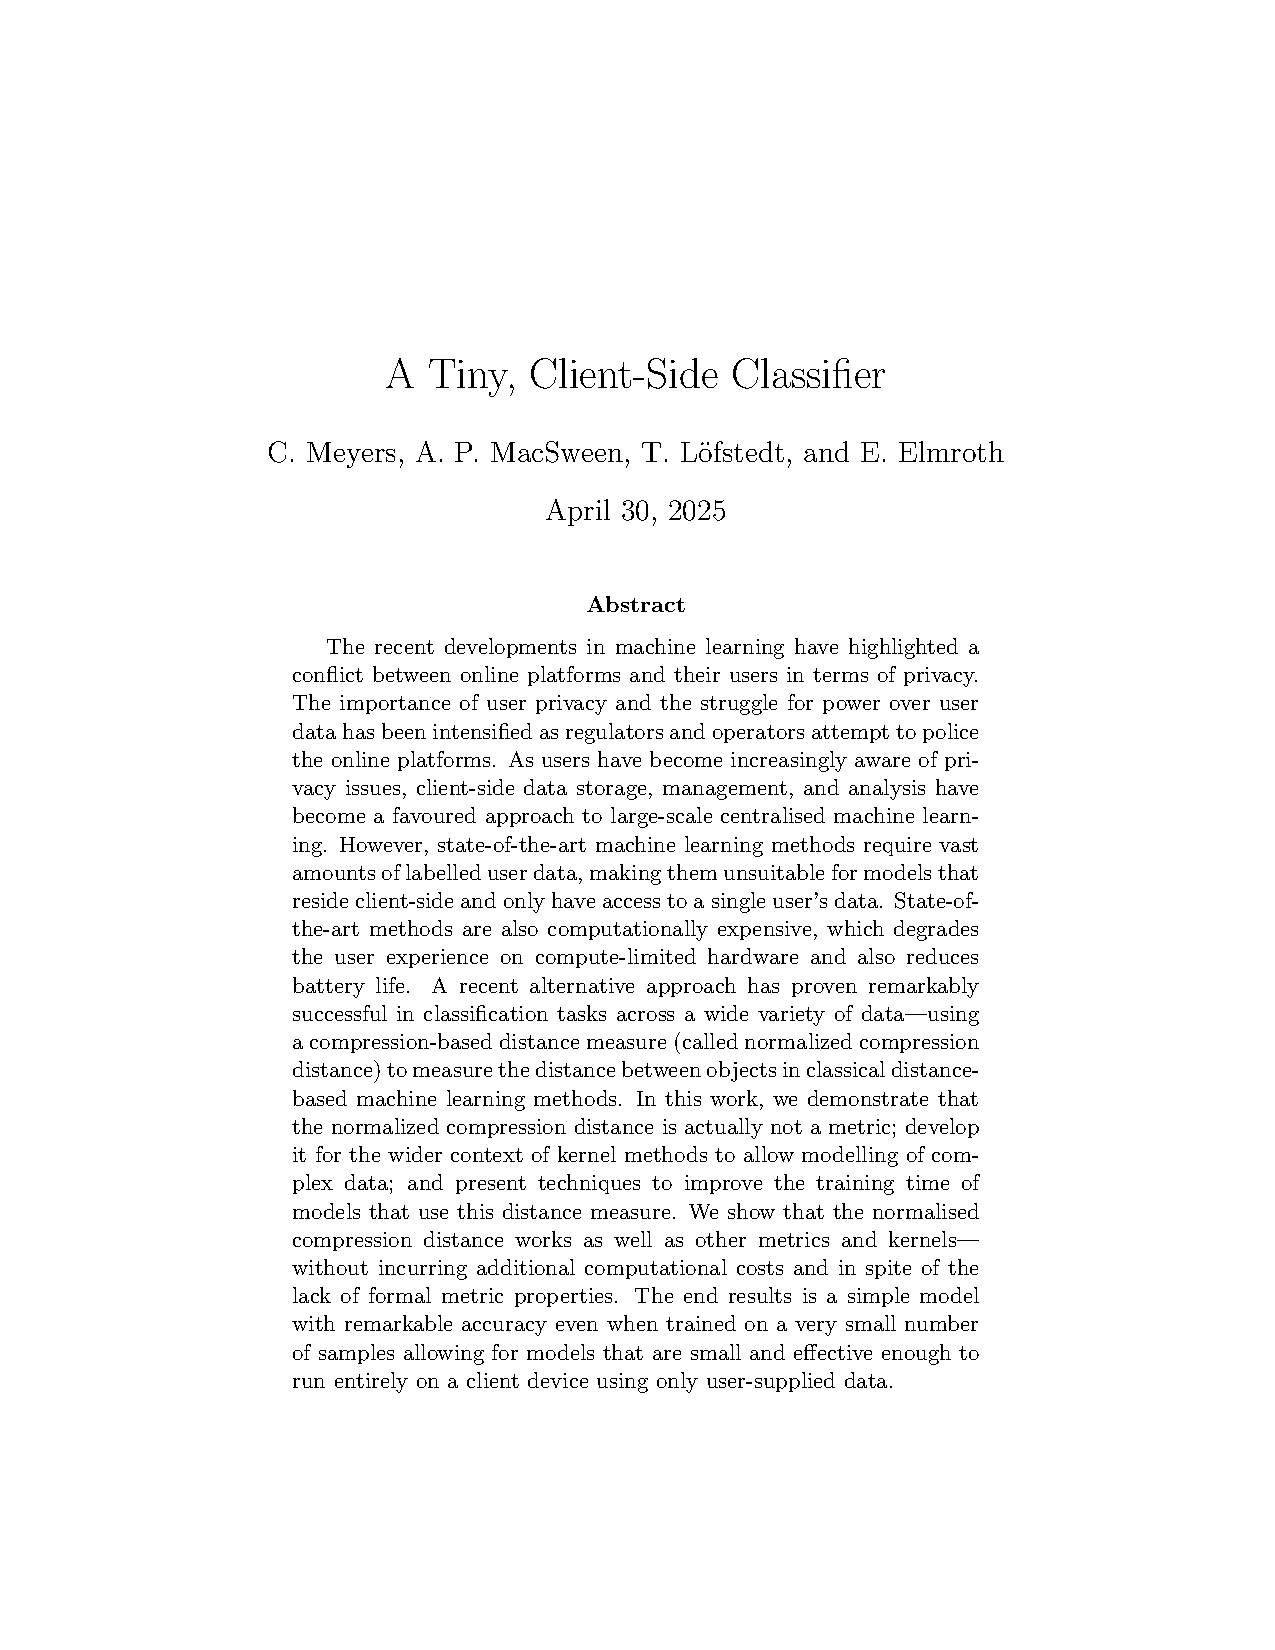
\includepdf[pages=-, pagecommand={}]{papers/Paper5.pdf}
\clearpage
\clearpage\mbox{}\clearpage %%EMAD USE IF ODD NUMBER OF PAGES PRECEDING
\thispagestyle{empty}
\raisebox{-30 mm }{
  \makebox[21cm]{
    \raggedleft                       
    \fontsize{24.88}{30} \bfseries Paper
    \colorbox{black}{
      \framebox[3cm][l]{
        \color{white}{\null\hspace{-3pt}VI}
        \rule[-8pt]{0pt}{36pt}        
      }
    }
  }
}
\vspace{-7pt}

\noindent
\rule[1mm]{412pt}{2pt}
\\{}\\ 
\PaperVI
\addcontentsline{toc}{chapter}{Paper VI}
\clearpage\mbox{}\thispagestyle{empty}\clearpage
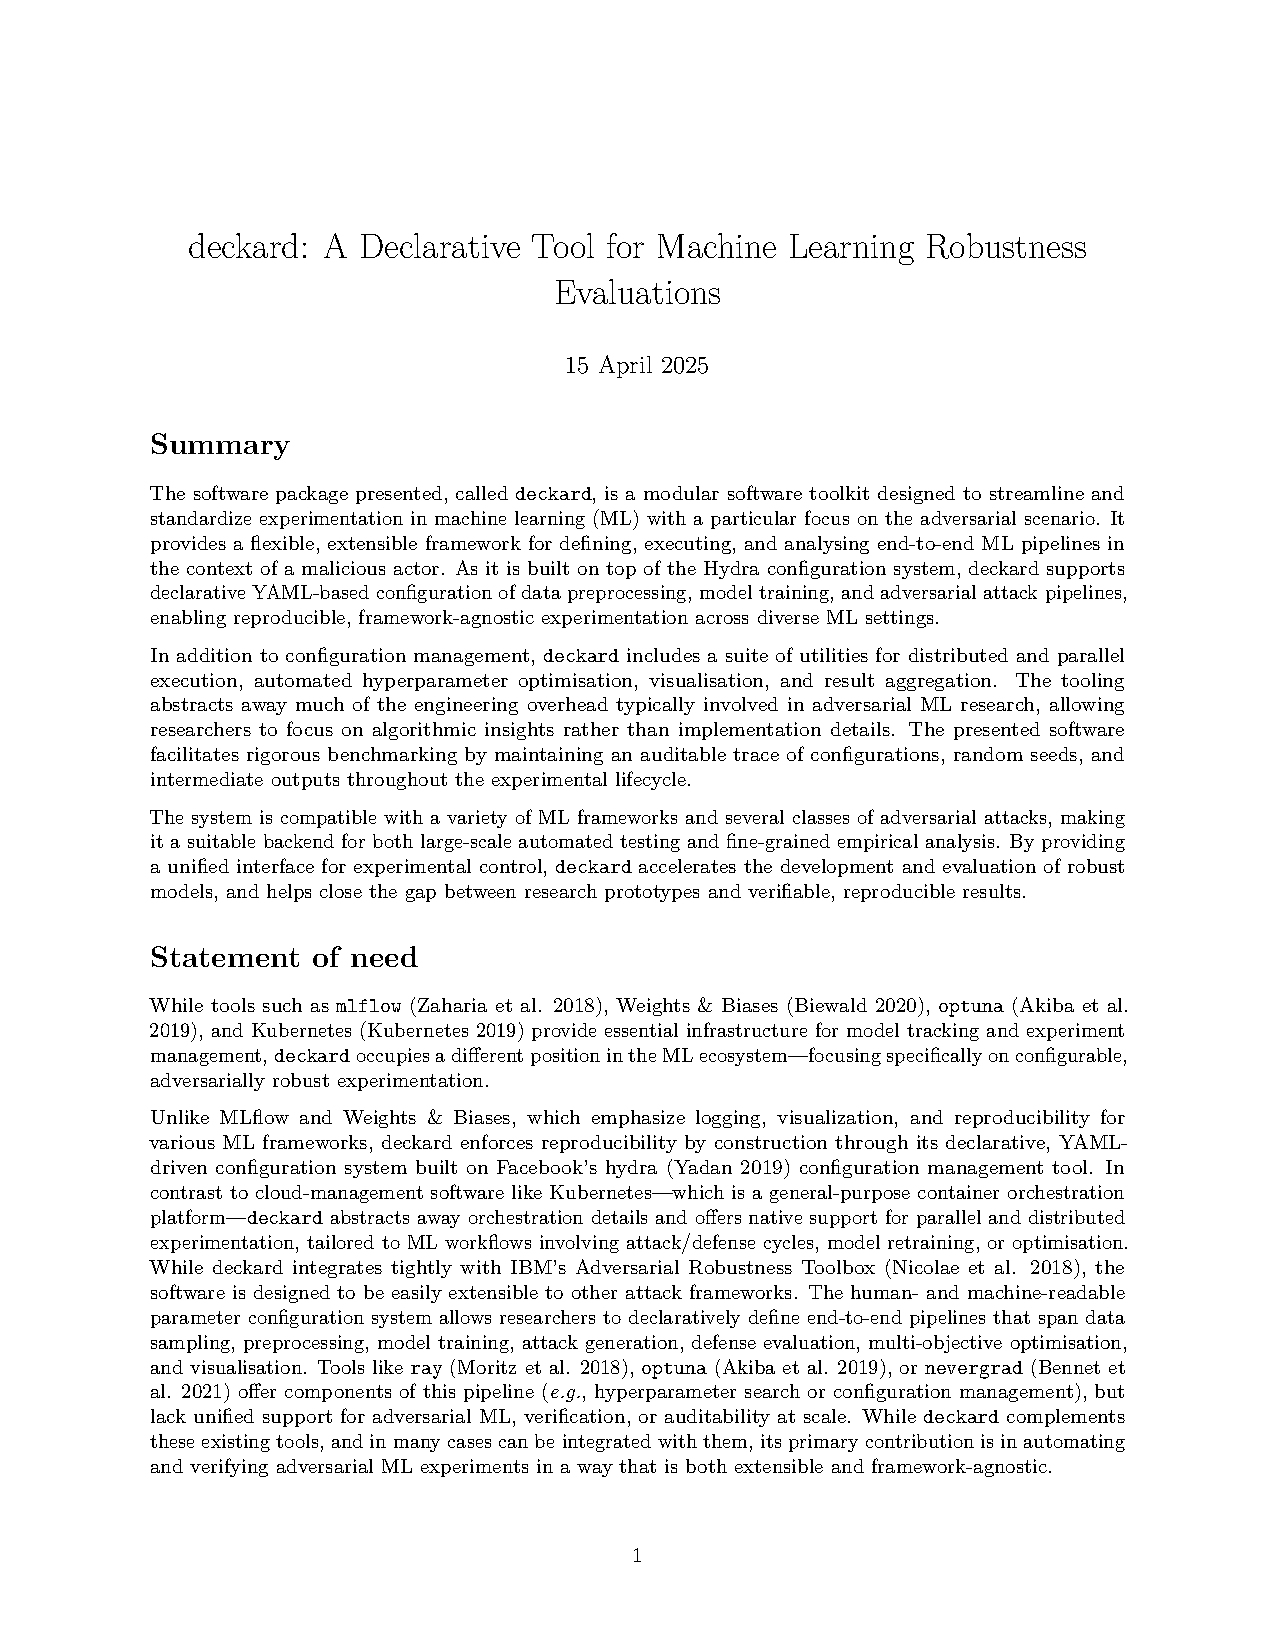
\includepdf[pages=-, pagecommand={}]{papers/Paper6.pdf}
\clearpage

% ------------------------------------------------------
%  Back Cover
% ------------------------------------------------------

\let\cleardoublepage\clearpage
\thispagestyle{empty}
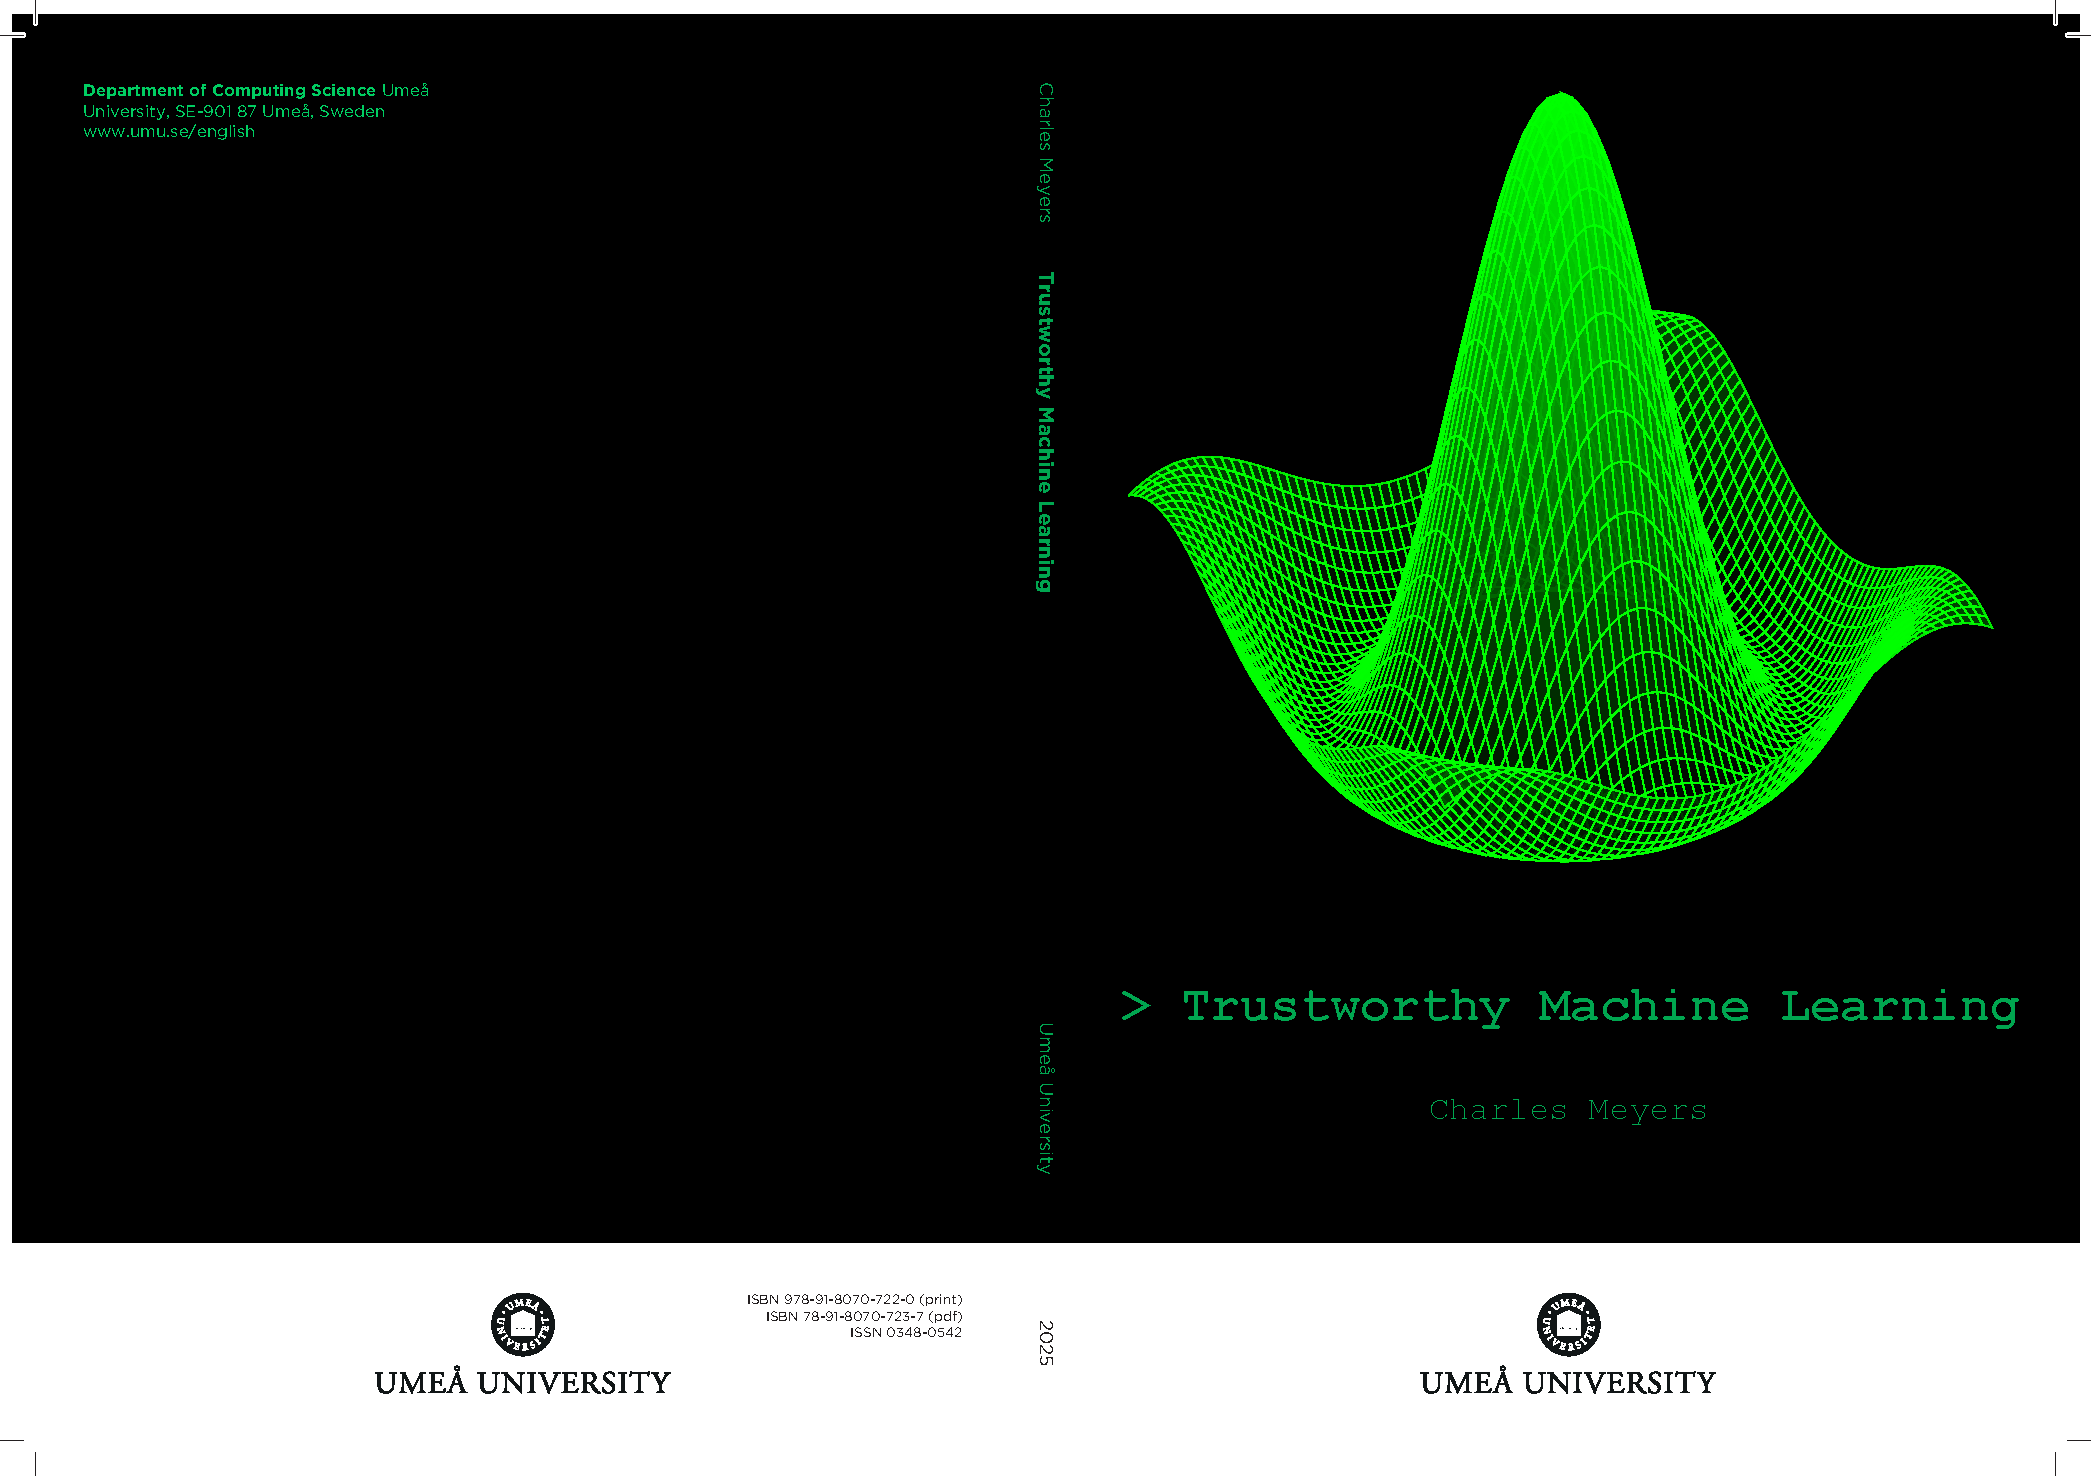
\includepdf[
  trim=5mm 5mm 180mm 5mm,
  clip,
  pagecommand={1},
  width=\paperwidth,
  height=\paperheight,
]{thesis_other_chapters/cover.pdf}
\thispagestyle{empty}
\end{document}